\documentclass[a4paper]{article}

\usepackage[utf8]{inputenc}
\usepackage[T1]{fontenc}
\usepackage{textcomp}
\usepackage{listings}
\usepackage{lmodern}
\usepackage{amsfonts}
\usepackage{titling}
\usepackage{lipsum}
\usepackage[left=1in, right=1in, bottom=1in, top=1in]{geometry}
\usepackage[backend=bibtex]{biblatex}
\usepackage{amsthm}
\usepackage{tcolorbox}
\usepackage{hyperref}
\usepackage{xcolor}
\usepackage{graphicx}
\usepackage{makeidx}
\usepackage{tikz}
\usepackage{cases}
\usepackage{apacite}
\usepackage{multirow}
\usepackage{tkz-berge}
\usepackage{lastpage}
\usepackage{fancyhdr}
\pagestyle{fancy} 
\usepackage{url}
\usepackage{tgtermes}
\usepackage{sectsty}
\usepackage{subcaption}
\usepackage{setspace}
\usepackage{float}
\usepackage{amsmath, amssymb}
\rhead{Page~\thepage~of~\pageref{LastPage}.}
\cfoot{}


% figure support
\usepackage{import}
\usepackage{xifthen}
\pdfminorversion=7
\usepackage{pdfpages}
\usepackage{transparent}
\newcommand{\incfig}[2][1]{%
    \def\svgwidth{#1\columnwidth}
    \import{./figures/}{#2.pdf_tex}
}

%mathstyling
\theoremstyle{plain}
\newtheorem{thm}{Theorem}[section]
\newtheorem{lem}[thm]{Lemma}
\newtheorem{prop}[thm]{Proposition}
\newtheorem*{cor}{Corollary}

\theoremstyle{definition}
\newtheorem{defn}{Definition}[section]
\newtheorem{conj}{Conjecture}[section]
\newtheorem{exmp}{Example}[section]
\newtheorem{axiom}{Axiom}
\theoremstyle{remark}
\newtheorem*{rem}{Remark}
\newtheorem*{note}{Note}

\pdfsuppresswarningpagegroup=1

\begin{document}
\begin{titlepage}
\begin{center}
\large
University of Warwick \\
Department of Computer Science \\
\huge
\vspace{50mm}
\rule{\linewidth}{0.5pt} \\
CS132 \\
\vspace{5mm}
\Large
Computer Organisation and Architecture
\rule{\linewidth}{0.5pt}
\vspace{5mm}
\begin{figure}[H]
\centering
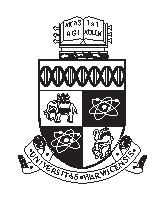
\includegraphics[width=0.4\textwidth]{crest_black.eps}
\end{figure}
\vspace{37mm}
Cem Yilmaz\\
\today
\end{center}
\end{titlepage}
\tableofcontents
\newpage

\section{C Programming}
\subsection{First programme}
Let us create a first programme that prints Hello world!
\begin{lstlisting}[language = C]
#include <stdio.h>
int main()
{
	printf("Hello world!/n")
	return 0;
}
\end{lstlisting}
In C, in order to execute libraries, we must use #include <name>. The standard I/O library is stdio.h and gives us access to printf function. \\
We also indicate that this is a main block of code by declaring our main to be int. Main function is always int.\\
We include /n to denote a newline, and we have to use return 0 in order to exit our function main.\\
In order to compile, we must find the location of our .c programme extension. After finding, type gcc -o name name.c in order to compile it. After, just type ./name into console. The -o creates an executable file of the name "name" using name.c.
\subsection{Data types}
There are 4 primitive data types in C:
\begin{lstlisting}[language = C]
char // 1 byte, 0 to 255 unsigned, -128 to 127 signed
int // 2 or 4 bytes, 0 to 6535 unsigned, -32768 to 32676 signed
float // 4 bytes, 32-bit IEEE single precision
double // 8 bytes, 64-bit IEEE double precision
\end{lstlisting}
Furthermore, you can use the $\%$ operator in order to specify what the print should be, e.g. integer, float etc.
\begin{lstlisting}[language = C]
%c // Character
%d // Signed integer
%e // Scientific notation of floats
%f // float value
%hi // Signed integer but short
%hu // Unsigned integer but short
%i // Unsigned integer
%l // long
%lf // Double
%Lf // long double
%s // string
%lu // unsigned long or int
%lli // long long
%llu // unsigned long long
%u // unsigned int
\end{lstlisting}

\subsection{Operators}
Binary arithmetic operators
\begin{lstlisting}[language = C]
+ // Addition
- // Subtraction
* // Multiplication
/ // Division
% // Remainder
\end{lstlisting}
Unary arithmetic operators
\begin{lstlisting}[language = C]
++ // adds +1 before or after depending on its location e.g. ++a
-- // subtracts 1 before or after depending on its location
\end{lstlisting}
Comparison operators
\begin{lstlisting}[language = C]
== // Is it equal to
< // less than
> // greater than
!= // not equal to
<= // less than or equal to
>= // greater than or equal to
\end{lstlisting}
Logical operators
\begin{lstlisting}[language = C]
& //  bitwise and
&& // logical and
| // bitwise or
|| // logical or
! // not
\end{lstlisting}
The difference between logical is that logical only takes in and returns boolean data type, whereas bitwise can take in integers as well and return the same data type.
\subsection{Loops}
\subsubsection{If statement}
The if statement in C is really similar to that in Java. Consider the following example:
\begin{lstlisting}[language = C]
#include <stdio.h>

int main() {
   int age = 20;
   
   if(age < 20)
   { 
      printf("You're still a teenager because you are %d\n", age);
   }
   else
   {
      printf("You're no longer a teenager because you are %d\n", age);
   }
}
\end{lstlisting}
\subsubsection{FOR loop (Bounded Iteration)}
A for loop is a loop which is done a fixed number of times.
\subsubsection{WHILE and DO-WHILE}

\section{Number Conversions}
\subsection{Binary}
\subsubsection{Binary to Octal}
We know that the binary system is represented by
\begin{align*}
	\sum_{n=0}^{k} a_n 2^{n}
\end{align*}
where $a_n \in\{0,1\}$
However, notice that, for the octal system represented by
\begin{align*}
	\sum_{n=0}^{k} b_n 8^n=\sum_{n=0}^{k} b_n 2^{3}^n
\end{align*}
This has several implications. What this means is that, for the coefficient $b_n$ in the octal system, which can go from 0 to 7, can be added from $3$ numbers in the binary. If we consider that $1111_2=15$, $1000_2=8$ and that $111_2 =7$, we can see that we can get coefficients for our base 8 number system we split up our number by 3 digits. This can be seen more clearly in the following example:
\begin{tcolorbox}[colback=black!3!white,colframe=black!60!white,title=\begin{exmp}Conversion 1 \label{Conversion 1}\end{exmp}]
        Convert $11101001101_2$ to base $8$.
	\begin{table}[H]
		\centering
		\label{tab:Conversion}
		\begin{tabular}{c|c|c|c}
		$011$ & $101$ & $001$ & $101$ \\
		$3$ & $5$ & $1$ &  $5$
		\end{tabular}
	\end{table}
		Therefore, it is $3515_8$
\end{tcolorbox}
\subsubsection{Binary to Hex}
With a similar principle,
\begin{align*}
	\sum_{n=0}^{k} c_n 16^n = \sum_{n=0}^{k} c_n 2^{4n}
\end{align*}
Similarly $11111_2=31$, $10000_2=16$ and $1111_2=15$, we can see how we can split up our binaries into 4 digits each to calculate the coefficients. We can again clearly see this in an example:
\begin{tcolorbox}[colback=black!3!white,colframe=black!60!white,title=\begin{exmp}Conversion 2\label{Conversion 2}\end{exmp}]
        Convert $110001110011011101_2$ to base $16$.
	\begin{table}[H]
		\centering
		\label{tab:conversion2}
		\begin{tabular}{c|c|c|c|c}
		$0011$ & $0001$& $1100$ & $1101$ & $1101$ \\
		$3$ & $1$ & $12$ & $13$ & $13$
		\end{tabular}
	\end{table}
	Therefore, it is $31CDD$
\end{tcolorbox}
\subsubsection{Signed Magnitude of Binary}
The signed magnitude of 2 bit is defined by the fact that the most left number, if $1$, will become negative. However, the rest of the coefficients will be negative.
\begin{tcolorbox}[colback=black!3!white,colframe=black!60!white,title=\begin{exmp}Signed Magnitude \label{Signed Magnitude}\end{exmp}]
Find $1100101_{2sm}$ in base $10$.\\

We notice that the number on the most left is $1$, Therefore our number must be negative. We now just have to compute $100101$ which is $2^6+2^2+1=$
                \begin{align}
			1100101_{2sm}=-37_{10}
                \end{align}
\end{tcolorbox}
The range of numbers for this number system can be found by $Numb \in [-2^{k-1}-1,2^{k-1}-1]$
\subsubsection{Two's Complement Representation of Binary}
The two's complement will also declare negative with the left most number, however, it does addition for each extra number. That is, the smallest number possible (the biggest negative) for a byte, is for example, $10000000_{2TC}=-128_{10}$ and $10000010_{2TC}=(-128+2)_{10}=-126_{10}$
\begin{tcolorbox}[colback=black!3!white,colframe=black!60!white,title=\begin{exmp}Finding Two Complement Numbers \label{Finding Two Complement Numbers}\end{exmp}]
Find $-9$ in a byte of a system in two complement.
                \begin{align}
		&9_{10}=1001_2\\
		\text{Ensure enough bits: }& 00001001_2\\
		\text{Invert:} & 11110110_2\\
		\text{Add 1:} & 11110111_2\\
		\implies & -9_{10} = 11110111_{2TC}
                \end{align}
		Note that there is also a second method: subtract $1$ and then invert. Both of these methods work for any number.
\end{tcolorbox}
 Furthermore, the range of two complements for some base $b$ is $b \in [b^{k-1},b^{k-1}-1]$
 \begin{tcolorbox}[colback=black!3!white,colframe=black!60!white,title=\begin{exmp}Find the range \label{Find the range}\end{exmp}]
 Find the range of a number represented by $abcd,efgh,ijkl_{2TC}$. 
                 \begin{align}
			 Numb \in [-2^{11}, 2^{11}-1]
                 \end{align}
 \end{tcolorbox}
\subsubsection{Fixed Point Representation of Binary}
We know in the number system we go in powers of $2$. Therefore, $0.11_2$ would represent $2^{-1}+2^{-2}$ in base $10$. This, however, it requires a lot of bits because you need a lot of numbers to represent specific decimals.
\subsubsection{Floating Point Representation}
The floating point representation is similar to the scientific notation, it used the same principles. All numbers are expressed in the form
\begin{align*}
	sign \cdot mantissa \cdot b^{\text{biased exponent}}
\end{align*}
Where mantissa represents the detail of the value to a certain precision; \\
The exponent represents the magnitude of the value. Note that the biased component is calculated by $\text{biased exponent}=\text{exponent}-(2^{k-1}-1)$ where $k$ is the amount of digits. This allows for negative numbers. Therefore, it follows that the $\text{biased exponent} \in [-b^{k-1}+1,b^{k-1}] \cap \mathbb{Z}$. and $b$ represents the base. In computers it's almost always $2$.
\begin{tcolorbox}[colback=black!3!white,colframe=black!60!white,title=\begin{exmp}Base 10 \label{Base 10}\end{exmp}]
Given that IEEE $754$ is expressed 1 bit for sign, 23 bits for mantissa and 8 bits for exponent, express $-12345_{10}$ in IEEE $754$ base $2$. $\implies$ Our sign is 1 as it is negative. 

                \begin{align}
			&12345_{10}=11000000111001_2  \\
			\implies & 1.1000000111001 \cdot 2^{13}\\
			\implies & \text{Mantissa}=10000001110010000000000 \\
				 &\text{Note that we add more $0 $s to the mantissa for 23 bits}\\
			\implies & 13+127=140\\
			\implies & 140_{10}=10001100_2\\
				 & \text{Ensure that the exp is 8 bits.}
                \end{align}
		Therefore our final answer is
		\begin{align}
		1100011001000000111001
		\end{align}
\end{tcolorbox}
\subsubsection{IEEE Floating Point}
IEEE Standard 754 is widely used and specifies levels of binary precision.\\
Single precision (uses 32 bits)\\
Double precision (using 64 bits) \\
Quad precision (using 128 bits) \\
For example, single precision uses 1 bit for the sign, 8 bits for the exponent and 23 bits for the mantissa.
\section{Logic and circuits}
\begin{figure}[H]
	\centering
	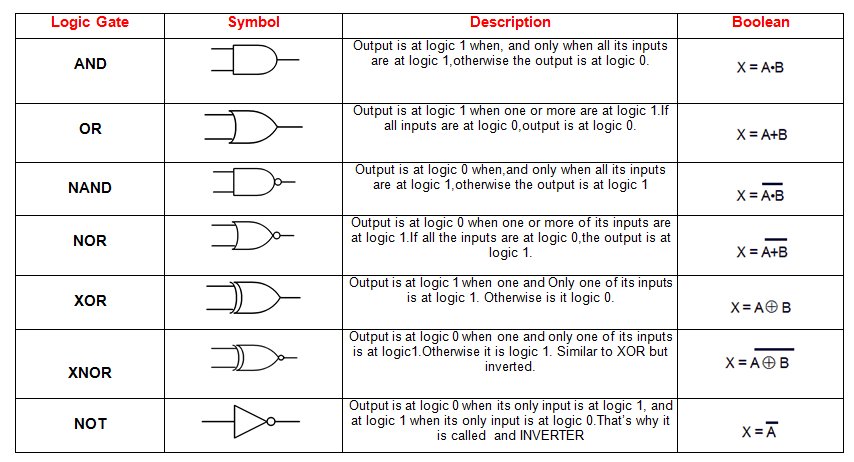
\includegraphics[width=0.8\textwidth]{logic.png}
	\caption{Logic gates}
	\label{fig:logic-png}
\end{figure}
It is sufficient to learn 4 gates: OR, AND, NOT and XOR. Rest are intuitive in symbol. You can also simplify boolean expressions using boolean logic or using karnaugh maps.
\subsection{Simplifying Circuits}
When given a function we need to be able to create equivalent circuits to meet several design criteria. These are:
\begin{enumerate}
	\item Perform the designated function\\
	\item Use the types of gates available \\
	Minimise the number of gates used and hence cost 
\end{enumerate}
\subsection{Karnaugh Maps (K-maps)}
Karnaugh maps are tables which consider $2$D truth tables. You would first construct a truth table for all the variables, and then map them onto the K-map. For example,
\begin{figure}[H]
	\centering
	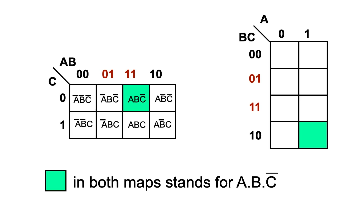
\includegraphics[width=0.42\textwidth]{figures/k1.png}
	\caption{Karnaugh Maps for triple variables}
	\label{fig:figures-k1-png}
\end{figure}
Notice that these are "gray coded", which means that adjacent variables only differ by 1 boolean expression. That is,
\begin{figure}[H]
	\centering
	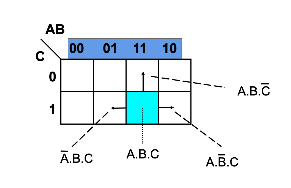
\includegraphics[width=0.3\textwidth]{figures/k2.png}
	\caption{Gray coded K-map}
	\label{fig:graycode}
\end{figure}
The first thing to also notice is the wrap around of Karnaugh maps. That is, in the figure below
\begin{figure}[H]
	\centering
	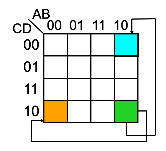
\includegraphics[width=0.2\textwidth]{figures/k3.png}
	\caption{K-map Wrapping}
	\label{fig:figures-k3-png}
\end{figure}
The bottom right green shaded square is actually adjacent to the other shaded corner squares. The top right is only adjacent to the bottom right, whereas the bottom left is only adjacent to also the bottom right.\\
The second thing to take note of is that K-maps are minimised when the number of groups (note that groupings must contain $2^{n}$ elements) that are identified are also minimal.
\begin{figure}[H]
	\centering
	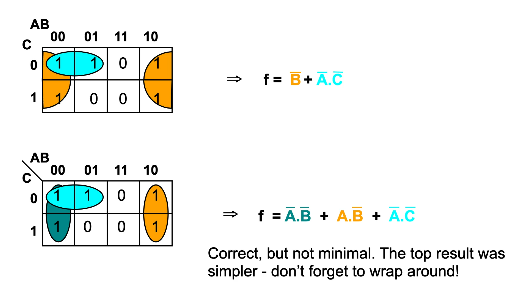
\includegraphics[width=0.6\textwidth]{figures/k4.png}
	\caption{Grouping}
	\label{fig:figures-k4-png}
\end{figure}	
In the first K-map, we notice in that in the orange circle that $\overline{B}$ does not change, therefore we can write it. Similarly, in the teal colour, we notice that $\overline{AC}$ does not change, therefore we can also write it. \\
In the second example, we have 3 examples, which work, but it is not minimal! \\
You can also have "Don't care conditions" which are denoted by red $x$, where we do not care about a specific square's value.
\subsection{Bit Adder}
A bit adder is a logical circuit which has a carry on and a sum of 3 inputs. The sum 'S' functions by checking the number 
\begin{figure}[H]
	\centering
	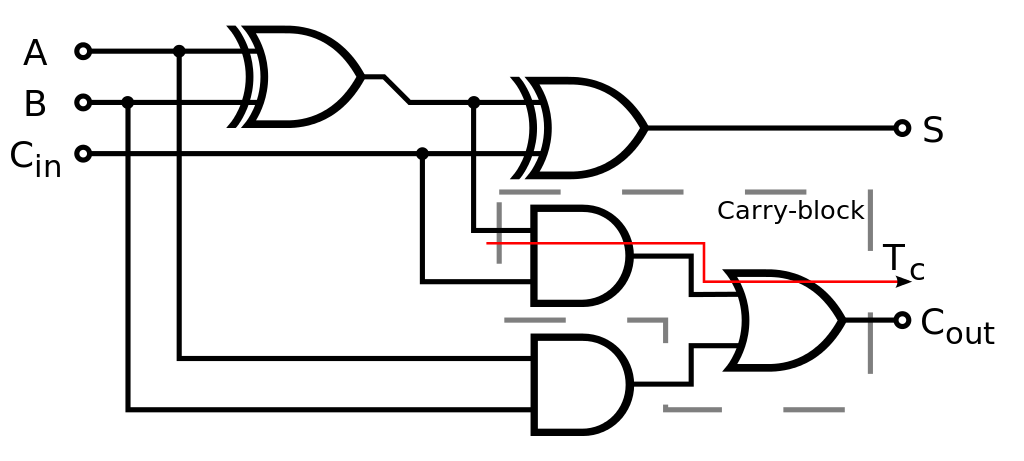
\includegraphics[width=0.6\textwidth]{figures/bitadder.png}
	\caption{Bit adder circuit}
	\label{fig:adder}
\end{figure}
\begin{table}[H]
	\centering
	\caption{Full Adder Truth Table}
	\label{tab:addertable}
	\begin{tabular}{c|c|c|c|c}
	\multicolumn{3}{c|}{Inputs} & \multicolumn{2}{c}{Outputs}\\
	\hline
	$A$ & $B$ & $C _{in}$ & $C_{out}$ & $S$ \\
	\hline
	0 & 0 & 0 & 0 & 0 \\
	0 & 0 & 1 & 0 & 1 \\
	0 & 1 & 0 & 0 & 1 \\
	0 & 1 & 1 & 1 & 0 \\
	1 & 0 & 0 & 0 & 1 \\
	1 & 0 & 1 & 1 & 0 \\
	1 & 1 & 0 & 1 & 0 \\
	1 & 1 & 1 & 1 & 1 \\
	\hline
	\end{tabular}
\end{table}
\subsubsection{$N$-bit adder}
Notice that the above only supports 2 bits of entry. We can, however, support multiple bits by combining 2 bits. That is, by combining $\times 2$ 2 bits. By having an $N$ number of bit adders combined, we achieve $N$ bit adders.
\begin{figure}[H]
	\centering
	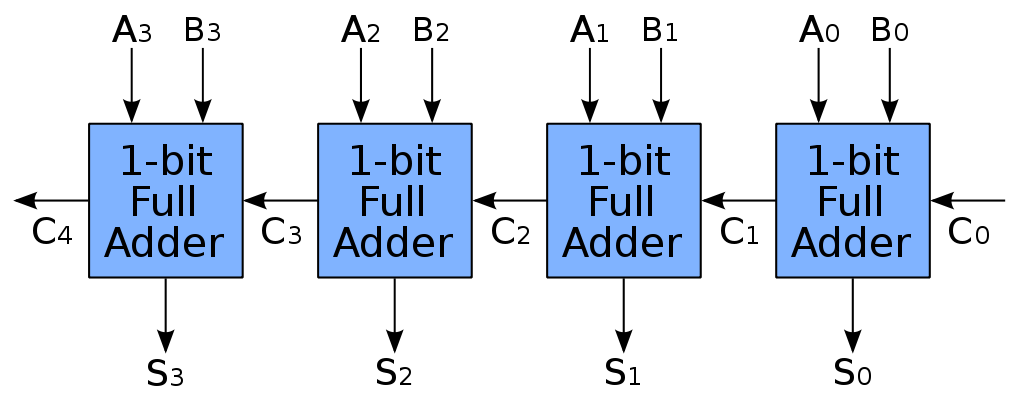
\includegraphics[width=0.5\textwidth]{figures/4bit.png}
	\caption{4 Bit adder}
	\label{fig:figures-4bit-png}
\end{figure}	
\subsubsection{Representing negatives}
We can do this by introducing two-complement circuit $Z$. \\
\begin{align*}
	Z = 0 &\implies S = A + B \\
	Z = 1 &\implies S = A - B 
\end{align*}
We can convert the bit adder to also do negatives by introducing two's complement. As we know,
\begin{enumerate}
	\item Invert the $N$-bit number $B$ by finding $Z \oplus B$.
	\item Add $1$ (Carry in)
\end{enumerate}
\begin{table}[H]
	\centering
	\caption{Z switch}
	\label{tab:Z}
	\begin{tabular}{cc|cc}
	$Z$& $B$ & \multicolumn{2}{c}{Result} \\
	 \hline
	 0 & 0 & 0 & \multirow{2}{*}{$=B$}\\
	 0 & 1 & 1 \\
	 \hline
	 1 & 0 & 1 & \multirow{2}{*}{$=\overline{B}$} \\
	 1 & 1 & 0 \\
	 \hline
	\end{tabular}
\end{table}
\begin{figure}[H]
	\centering
	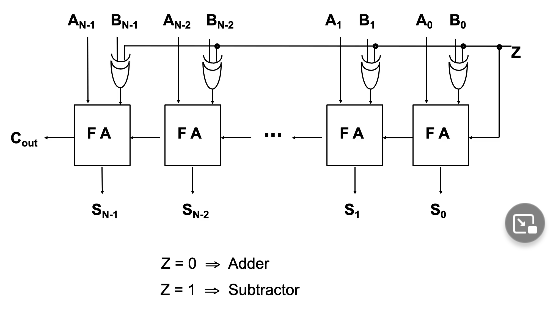
\includegraphics[width=0.6\textwidth]{figures/subtractor.png}
	\caption{Subtractor}
	\label{fig:figures-subtractor-png}
\end{figure}
As from the previous thing we've discussed, the $+1$ is from the fact that if $Z=1 $, the input is already added $1$ ! Note that this does not directly add to $B$, but this is fine as the $+1$'s position does not matter. 
\subsection{Active and Inactive states}
Circuits can be defined using "active" and "inactive" states, which can change the meaning of the values $0$ and $1$. 
\subsubsection{Active High}
In active high, it follows that:
\begin{align*}
	0 &= \text{inactive} \\
	1 &= \text{active}
\end{align*}
\subsubsection{Active low}
In active low, it follows that:
\begin{align*}
	0 &= \text{active} \\
	1 &= \text{inactive}
\end{align*}
\subsection{Decoder}
A decoder is a circuit such that for $n$ amount of entries, it will have $2^{n}$ amount of outputs to count in for each possibility. It follows that, the addition of the entries will in fact determine in which row the $0$ will take place in. The description is more clear when noticed in the figure below:
\begin{figure}[H]
    \centering
    \incfig[0.5]{decoder}
    \caption{$2 \times 4$ Decoder}
    \label{fig:decoder}
    Note that this is a high active binary decoder.
\end{figure}
\subsection{Encoder}
Encoder does the exact opposite of a decoder. In some sense, it takes $2^{n}$ inputs, and has $n$ amount outputs.
\begin{figure}[H]
    \centering
    \incfig[0.5]{encoder}
    \caption{Encoder}
    \label{fig:encoder}
\end{figure}
\subsection{Multiplexer}
In multiplexers, output is a selected input. The sum of the gates determine the value of this customised input.
\begin{figure}[H]
	\centering
	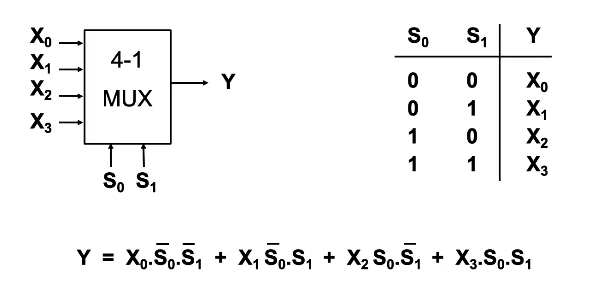
\includegraphics[width=0.5\textwidth]{figures/multiplexer.png}
	\caption{4 to 1 Multiplexer}
	\label{fig:figures-multiplexer-png}
\end{figure}
\subsection{De-Multiplexer}
In de-multiplexers, you allow one of the outputs to be any one of the outputs.
\begin{figure}[H]
	\centering
	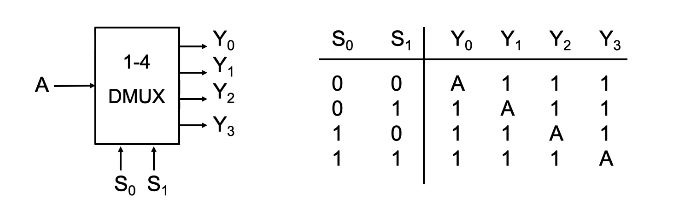
\includegraphics[width=0.5\textwidth]{figures/demultiplexer.png}
	\caption{De-multiplexer}
	\label{fig:figures-demultiplexer-png}
\end{figure}
\subsection{Sequential Logic}
A logic circuit whose outputs are logical functions of its inputs and its current state.
\subsubsection{Flip-Flops}
Flip flops are a circuit whose outputs are fed back to inputs. In an active low flip flop, the set and reset have a bar over them. Furthermore, when set bar is set to 0, Q is set to 1. When reset is set to 0, Q is set back to 0. Note that $\neg P = Q$. 
\begin{figure}[H]
	\centering
	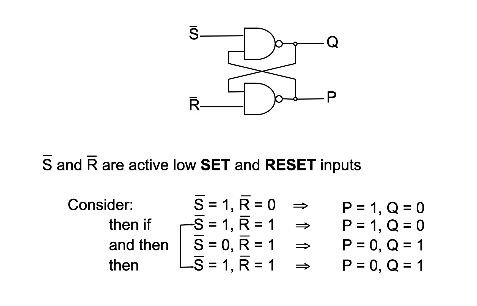
\includegraphics[width=0.5\textwidth]{figures/flip.png}
	\caption{Active Low Flip-Flop}
	\label{fig:figures-flip-png}
\end{figure}	
Essentially, $Q$ is set to one when $\overline{S}=0$ (and $\overline{R}=1$ )\\
And $Q$ is Reset (to zero) when $\overline{R}=0$ (and $\overline{S}=1$ ). \\
If $\overline{S}=\overline{R}=1$, then $Q$ does no change. \\
However, when $\overline{S}=\overline{R}=0$, we get a hazard condition.
\subsection{D-Type Latch}
Using a modified form of the flip-flop circuit we've seen it is possible to design the D-type latch, which is essentially a 1-bit memory circuit.
\begin{figure}[H]
	\centering
	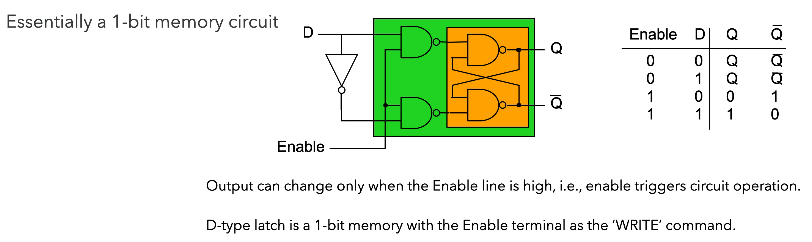
\includegraphics[width=0.8\textwidth]{figures/latch.png}
	\caption{D-Type Latch}
	\label{fig:figures-latch-png}
\end{figure}
In the figure above, $D$ is a 1-bit data that is either $0$ or $1$. The value of $D$ is stored into $Q$ if and only if Enable is  $1$. 
\begin{table}[H]
	\centering
	\caption{D-Type Latch Truth Table 1}
	\label{tab:table1}
	\begin{tabular}{cc|cc}
	Enable & $D$ & $Q$ & $\neg Q$ \\
	\hline
	$ 0$ & $x$ & $Q$ & $\neg Q$ \\
	$1$ & $0$ & $0$ & $1$ \\
	$1$ & $1$ & $1$ & $0$ \\
	\hline
	\end{tabular}
\end{table}
\begin{table}[H]
	\centering
	\caption{D-Type Latch Truth Table 2}
	\label{tab:table2}
	\begin{tabular}{cc|cc}
	Enable & $D$ & $Q$ & $\neg Q$ \\
	\hline
	$0$ & $0$ & $Q$ &  $\neg Q$ \\
	$0$ & $1$ & $Q$ & $\neg Q$ \\
	$1$ & $0$ & $0$ & $1$ \\
	$1$ & $1$ & $1$ & $0$ \\
	\hline
	\end{tabular}
\end{table}
\begin{table}[H]
	\centering
	\caption{D-Type Latch Truth Table 3}
	\label{tab:table3}
	\begin{tabular}{c|cc}
	Enable & $Q$ & $\neg Q$ \\
	\hline
	$0$ & $Q$ & $\neg Q$ \\
	$1$ & $D$ & $\neg D$ \\
	\hline
	\end{tabular}
\end{table}
\subsection{Clocked Flip-Flops}
In some cases, $D$-type is a special case of a flip-flop in which the enabler is a clock. That is, the clock only outputs true when the clock is 'rising', i.e. transitioning from low to high. There are many circuits in which a clocked flip-flop is used, most of which that are relevant for the module can be found in the figure below:
\begin{figure}[H]
	\centering
	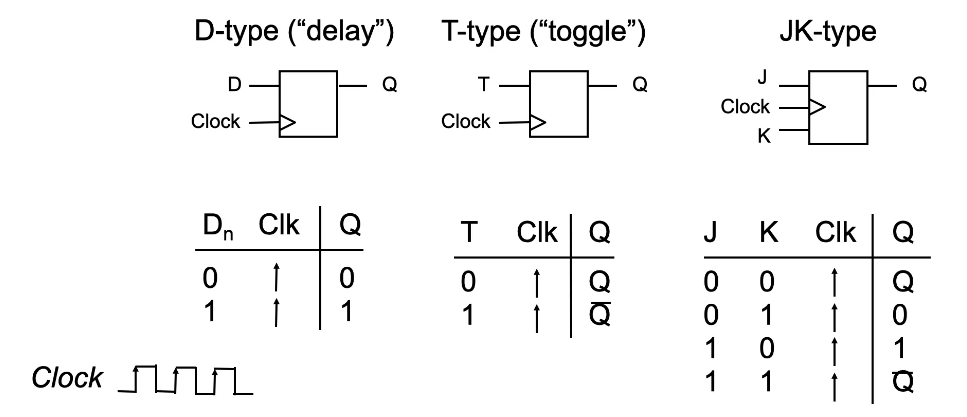
\includegraphics[width=0.8\textwidth]{figures/clocked.png}
	\caption{Examples of Clocked Flip-Flops}
	\label{fig:figures-clocked-png}
\end{figure}
However, the module will primarily be focusing on $D$-type.
\subsection{N-bit Register}
An N-bit register is a multi-bit memory that allows us to store $n$ bits using a $D-$type latch. 
\begin{figure}[H]
	\centering
	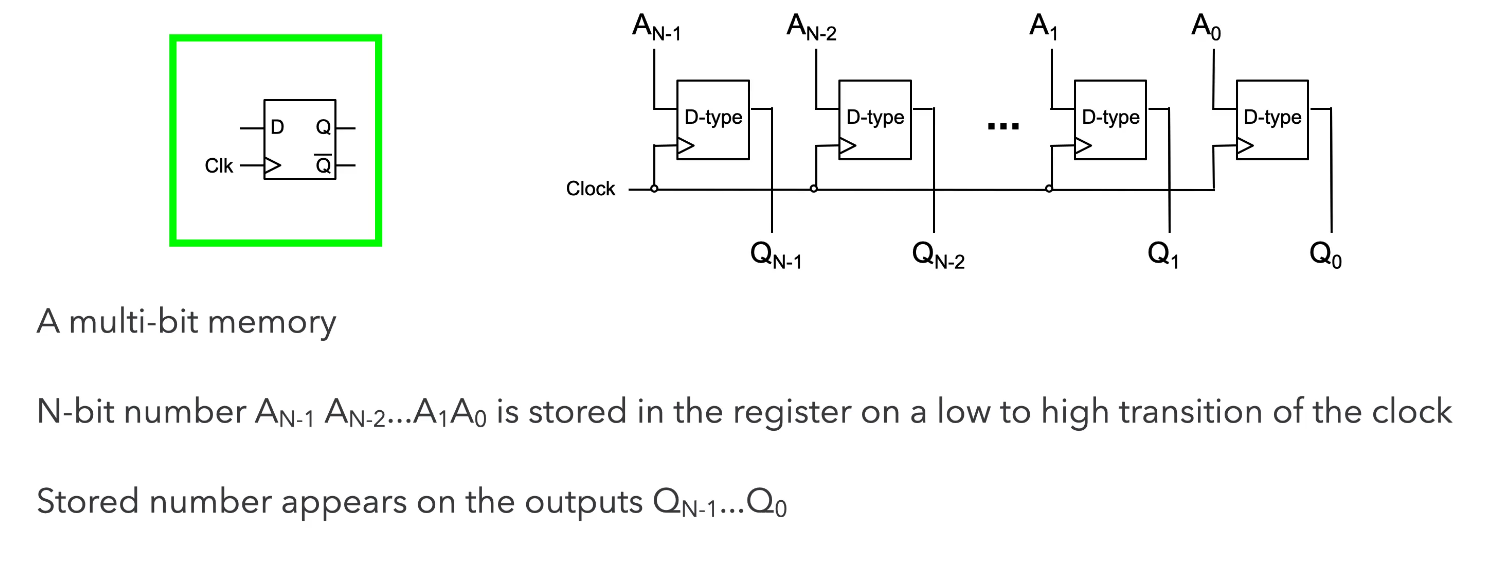
\includegraphics[width=0.8\textwidth]{figures/register.png}
	\caption{Parallel Load N-bit Register}
	\label{fig:figures-register-png}
\end{figure}
\subsection{N-bit Shift Register} 
The important part of this register is that once the clock is ran once, the input of $D$ will go to $Q_{N-1}$ and will be stored there. Then, we can change the input $D$ again and store that in $Q_{N-1}$ and store the old $Q_{N-1}$ in $Q_{N-2}$ once we run the clock again. 
\begin{figure}[H]
	\centering
	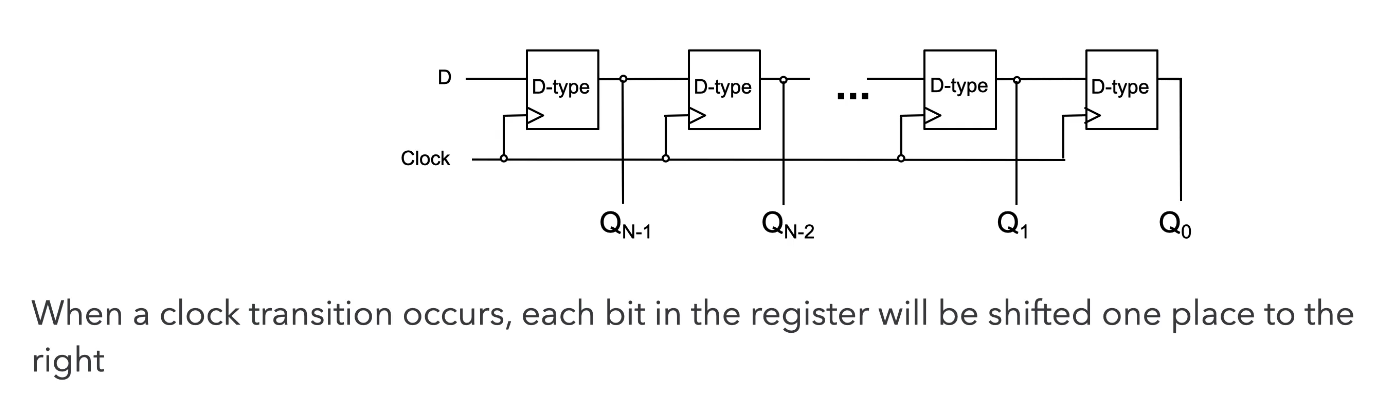
\includegraphics[width=0.8\textwidth]{figures/shift.png}
	\caption{N-bit Shift Register}
	\label{fig:figures-shift-png}
\end{figure}
\subsection{N-bit Counter}
The N-bit Counter is a complex circuit.
\begin{figure}[H]
	\centering
	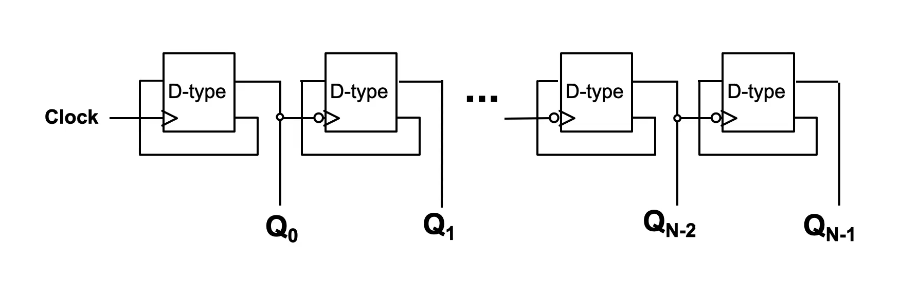
\includegraphics[width=0.8\textwidth]{figures/counter.png}
	\caption{N-bit Counter}
	\label{fig:figures-counter-png}
\end{figure}
One thing to note is that the triangle with the circle denotes an inverter, that is, it is a clock that only registers when a value drops. Let us run this circuit 3 times to see the logic behind it.
\subsubsection{First run}
We first begin with the fact that we are at $000$. That is, each $Q=0$. Now, let us switch the clock and we get a $1$ in the input for the enabler. Because $Q_0=0$, $\neg Q_0=1$, therefore our inputs into our first D-type are $1$ and $1$. Then, the D-type stores the $1$ into $Q_0$. Then, our new $\neg Q_0=0$, which is fed back into the D-type. Note that it stops here, because we have increased our value from $0$ to $1$ for $Q_0$, therefore the inverter does not function.
\subsubsection{Second run}
In the second run, we insert a $1$ again. Our $D-type$ has the inputs $0$ and $1$, which means that $Q_0$ is now a $0 $. Since $Q_0$ has dropped in value, the inverter clock on the second D-type was triggered, which now has inputs of $1$ and $1$, setting $Q_1=1$.
\subsubsection{Third Run}
The third run is similar to the first. We run the clock and we get the inputs $1$ and $1$, which sets $Q_0$ to $1$, and does not proceed.
\subsection{Three-state Logic}
The logical components we've considered so far had only $0 $ and $ 1$. There is another gate, called the three-state buffer, whose output can be placed in a third state defined as 'UNCONNECTED'
\begin{figure}[H]
	\centering
	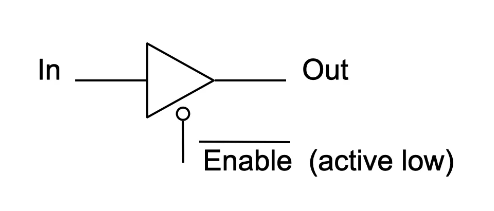
\includegraphics[width=0.3\textwidth]{figures/three.png}
	\caption{Three-state Logic}
	\label{fig:three-png}
\end{figure}
When $\overline{Enable}$ is high, the input is disconnected from the output \\
When $\overline{Enable}$ is low, the input is connected to the output
\subsection{Three-state Buses}
Consider a bus with an output that we want to share on multiple D-types. However, we cannot have multiple outputs at the same time. Thus, we use a three-state logic connected to our buses to give control lines. 
\begin{figure}[H]
	\centering
	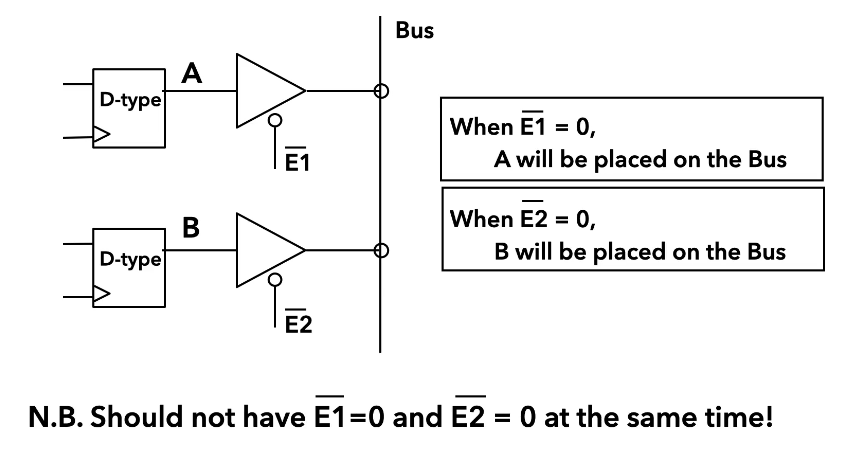
\includegraphics[width=0.5\textwidth]{figures/bus.png}
	\caption{1 Bit Three-state Bus}
	\label{fig:figures-bus-png}
\end{figure}
\subsection{N-bit Three-state Buses}
\begin{figure}[H]
	\centering
	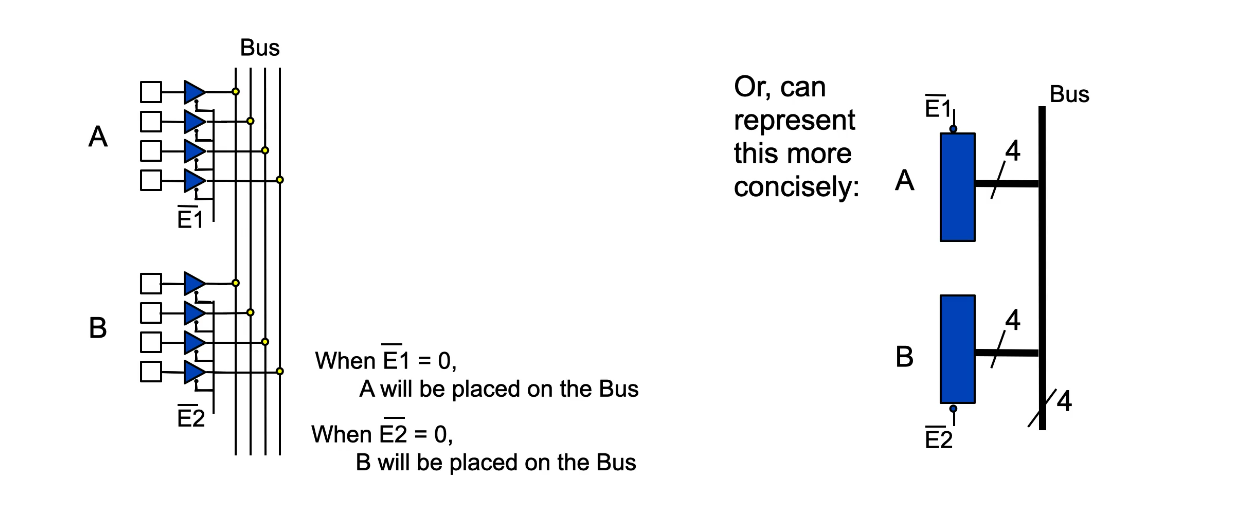
\includegraphics[width=0.8\textwidth]{figures/multibus.png}
	\caption{4-Bit Three-state Bus}
	\label{fig:figures-multibus-png}
\end{figure}
\subsection{Properties of Logic Gates}
The are several things to remember about how particular a $0$ or a $1$ is determined in a circuit, specifically that
\begin{figure}[H]
	\centering
	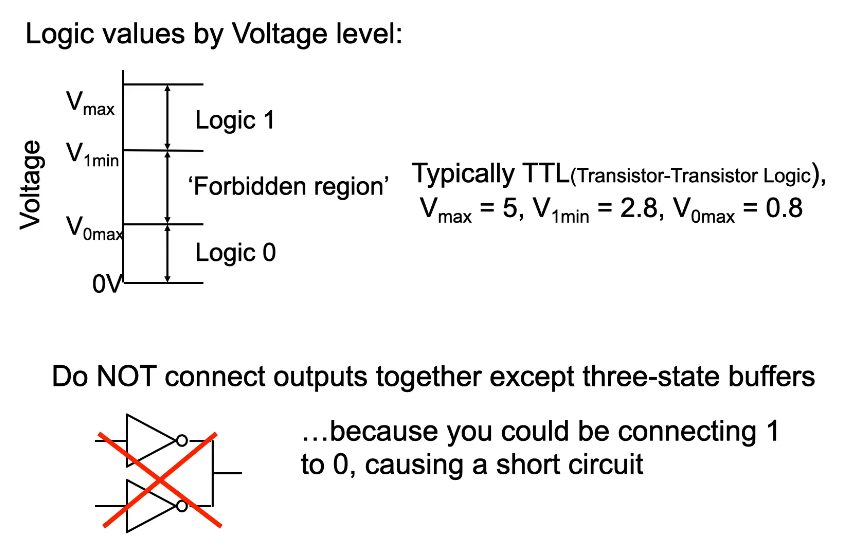
\includegraphics[width=0.6\textwidth]{figures/rules.png}
	\caption{Properties of Logic Gates}
	\label{fig:figures-rules-png}
\end{figure}
\subsection{Propagation Delay}
Each logic has a propagation delay, typically in nano-seconds, ($1 \times 10 ^{-9}$s or less, limiting the speeds of logic circuits. However, this can be reduced by ensuring logic gates are close together and are on the same integrated circuit.
\begin{table}[H]
	\centering
	\caption{Propagation Delay}
	\label{tab:delay}
	\begin{tabular}{c|c}
		Gate & Propagation Delay (ns) \\
		\hline
		NOT & $1.0$ \\
		NAND & $1.2$ \\
		AND & $1.7$ \\
		OR & $1.2$ \\
		NOR & $1.5$ \\
		\hline
	\end{tabular}
\end{table}
\section{Assembler}
\subsection{Microprocessor Fundamentals}
\subsubsection{Central Processing Unit (CPU)}
The CPUs control and perform instructions. They use two units that are the following:
\begin{enumerate}
	\item Arithmetic Logic Unit (ALU) - Performs mathematical and logical operations
	\item Control Unit (CU) - Decodes program instructions and handles logistics for the execution of decoded instructions.
	\item Program Counter - Tracks the memory address of the next instruction to be executed
	\item Instruction Register (IR) - Contains most recent instruction fetched
	\item Memory Address Register (MAR) - Contains address of the region of memory to be read or written, i.e. location of data to be accessed
	\item Memory Data Register (MDR) - Contains data fetched from memory or data to be written to memory. Also known as Memory Buffer Register.
\end{enumerate}
The CPU continuously performs instruction cycle. These are retrieved from memory, decoded to form recognisable operations and executed to impact the current state of CPU.
\subsubsection{Fetch-Decode-Execute Cycle}
It consists of the following:
Fetch
\begin{enumerate}
	\item Instruction retrieved from memory held by program counter
	\item Retrieved instruction stored in instruction register
	\item Program Counter incremented to point to next instruction in memory
\end{enumerate}
Decode
\begin{enumerate}
	\item Retrieved instruction / operation code / opcode decoded
	\item Read effective address to establish opcode type 
\end{enumerate}
Execute
\begin{enumerate}
	\item Control unit signals functional central processing unit components
	\item May result in changes to data registers, that is, the program counter, arithmetic logic unit, input/output etc.
\end{enumerate}
\subsection{68008 Architecture}
\subsubsection{Data Register}
D0-D7, 32 bit registers which can partition themselves to 8,16 as well, store frequently used values / intermediate results
Strictly speaking we would only require one register on a chip. The advantage of many data registers is that fewer references to external memory are required. Registers can be treated as long, word or byte, that is, 32 bits, 16 bits or 8 bits respectively.
\subsubsection{Status Register}
The status register is 16 bits, and consists of two 8-bit registers. It explains the current status of the processor, that is, where it is currently.
Its status bits are set or reset upon certain conditions or commands that happen in the ALU.
\begin{figure}[H]
	\centering
	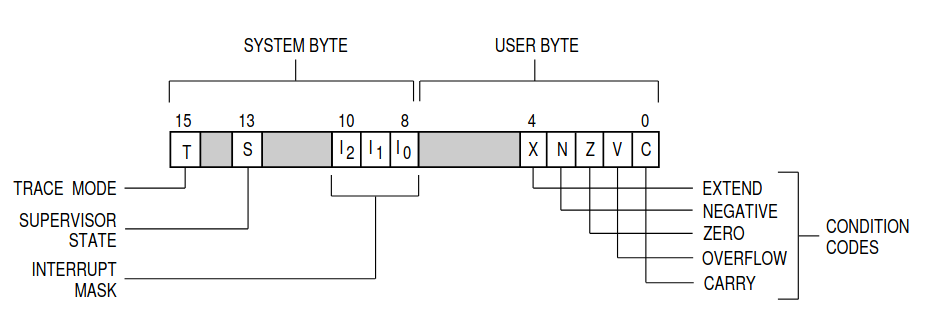
\includegraphics[width=0.8\textwidth]{figures/statr.png}
	\caption{Status Register}
	\label{fig:figures-statr-png}
\end{figure}	
\subsubsection{Address Register}
The Address Registers uses A0-A6, 32 bit registers. These store addresses that we may use for future operands. That is, we are able to return to a memory address that we previously were at. The A7 is additionally used by the processor as a system slack pointer to hold subroutine routine addresses etc. It is important to note that operations on addresses do not alter the CCR.
\subsubsection{Stack Pointer}
Stack is a type of architecture that stores the latest operations.\footnote{Tenenbaum p.250-268 is worthy of read to understand fully}. The stack pointer is essentially used in A7 of the Address Register. It is also possible to use A0-A6 was stack pointers if needed.
\subsubsection{Program Counter}
A 32 bit register that keeps track of the address at which the next instruction will be found. In simple terms, it points to the next instruction in memory.
\subsection{Register Transfer Language}
It is used to describe the set of operations of a microprocessor as it is executing instructions. E.g. $[MAR] \leftarrow [PC]$ means transfer of Program Counter to the Memory Address Register. The computer's main memory is called Main Store The contents of memory location 12345 is written $[MS\left( 12345 \right) ]$. It is important not to confuse register transfer language with assembler instructions.
\subsection{Instruction Cycle}
The RTL representation we will seem makes no attempt to account for the pipelining of instructions. Pipelining is a common and a simple method of speeding up the fetch-execute cycle.
\begin{figure}[ht]
    \centering
    \incfig{icycle}
    \caption{LFT Cycle}
    \label{fig:icycle}
\end{figure}
\subsubsection{Fetching}
\begin{enumerate}
	\item Contents of Program Counter transferred from MAR address buffers and the Program Counter is incremented
	\item MBR loaded from external memory ($R$/$\overline{W}$ line set to Read)
	\item Opcode transferred to Instruction Register from MBR
	\item Instruction is decoded
\end{enumerate}
In RLT, this is 
 \begin{enumerate}
	 \item $[MAR] \leftarrow [PC]$ 
	 \item $[PC] \leftarrow [PC]+1$
	 \item $[MBR] \leftarrow [MS([MAR])]$ ($R$ / $\overline{W}$ set to Read)
	 \item $[IR] \leftarrow [MBR]$
	 \item  $CU \leftarrow [IR(opcode)]$
\end{enumerate}
And it is the same for every instruction set.
\subsubsection{Decode}

\subsection{Assembly Language}
In coding, the hierarchy
\begin{figure}[ht]
    \centering
    \incfig{hierarchy}
    \caption{hierarchy}
    \label{fig:hierarchy}
\end{figure}
Follows. Assembly language can give you the control over instructions you give to your microprocessor. 
\subsubsection{Assembler format}
Assembly language vary but typically have similar format:\\
$<Label>:<OPCODE> \; <OPERAND(S)> \; | COMMENT$\\
e.g.\\
$START: \; move.b \; 5,D_0 |\text{Load D0 with 5}$
\begin{figure}[H]
	\centering
	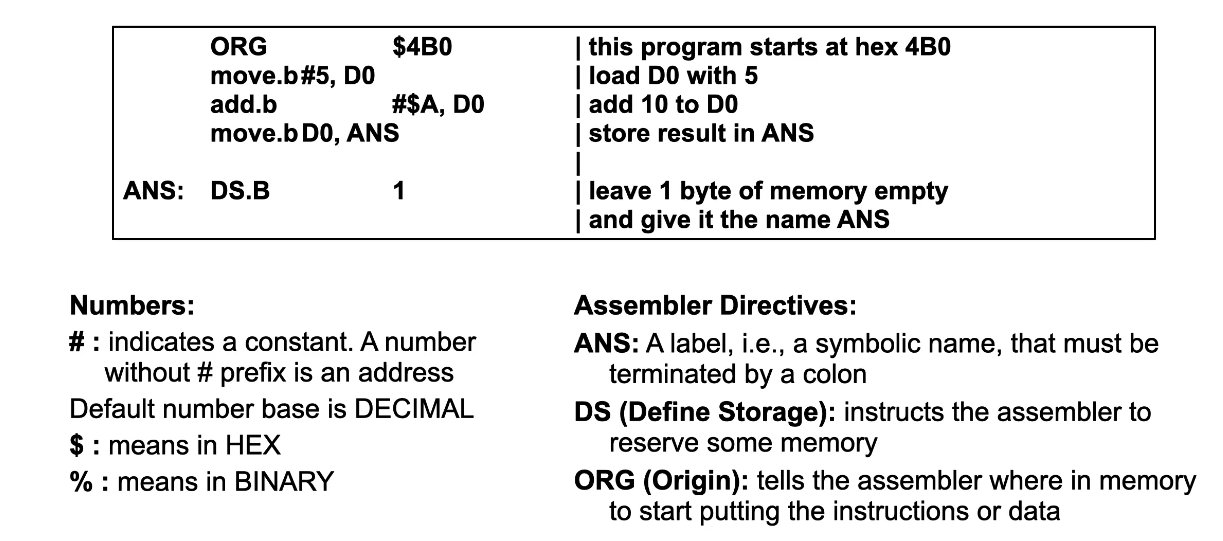
\includegraphics[width=0.8\textwidth]{figures/assem.png}
	\caption{Assembly Language}
	\label{fig:figures-assem-png}
\end{figure}
In other words, in $68008$ it is \\
$operation.datatype \; source, \;destination$ for movement.
\subsection{68008 Instructions}
The $68008$ instruction set is made up five categories of instructions:
\begin{enumerate}
	\item Data movement
	\item Arithmetic
	\item Logical
	\item Branch
	\item System Control
\end{enumerate}
For this course, the first four are sufficient.
\subsubsection{Data Movement}
Data instructions are written in the form
\begin{align*}
	operation.datatype \; source, \; destination
\end{align*}
The operation ca be on one of the three data types:
\begin{align*}
	byte \; \; .b \text{($8$ bits)} \\
	word \; \; .w \text{($2$ bytes)} \\
	long word \; \; .l \text{( $4$ bytes)}
\end{align*}
In default, the data type is word.
\begin{figure}[H]
	\centering
	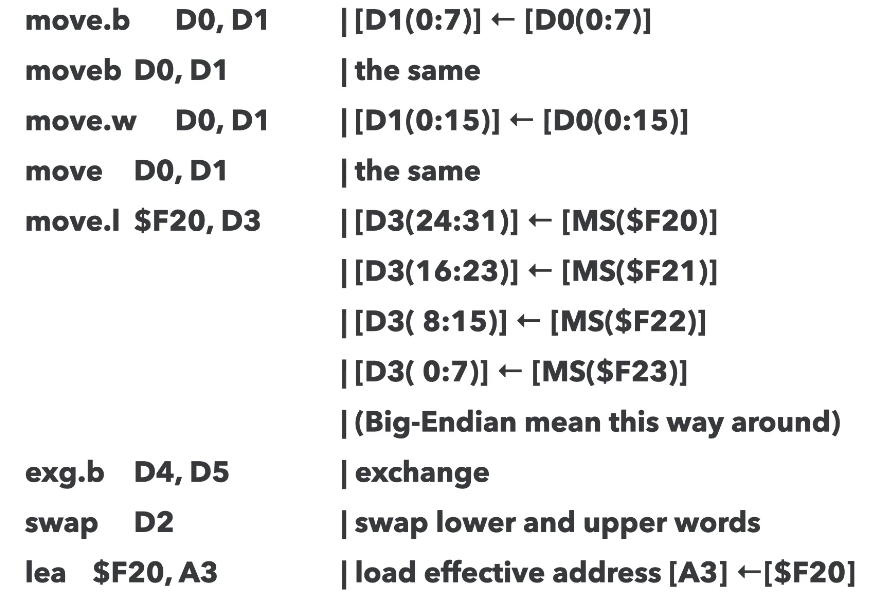
\includegraphics[width=0.6\textwidth]{figures/movement.png}
	\caption{I have 0 clue what the fuck this says}
	\label{fig:figures-movement-png}
\end{figure}
\subsubsection{Arithmetic Instructions}
\begin{figure}[H]
	\centering
	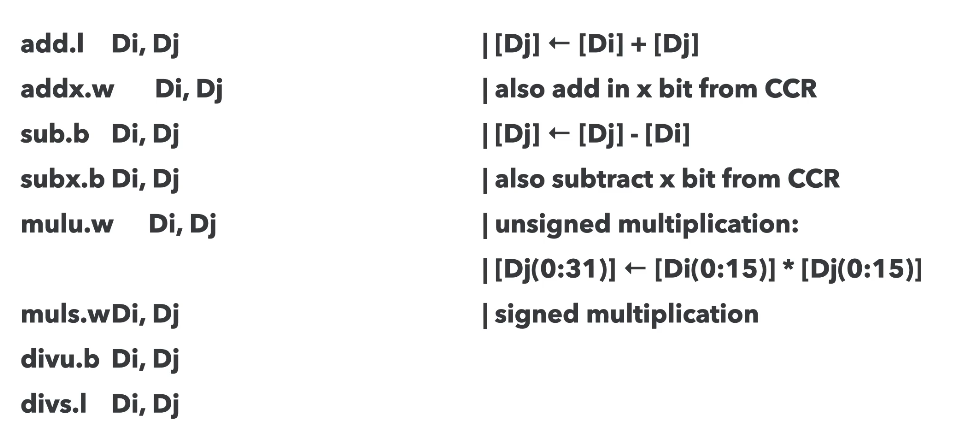
\includegraphics[width=0.8\textwidth]{figures/arinst.png}
	\caption{Arithmetic Instructions}
	\label{fig:figures-arinst-png}
\end{figure}
\subsubsection{Logical Instructions}
\begin{figure}[H]
	\centering
	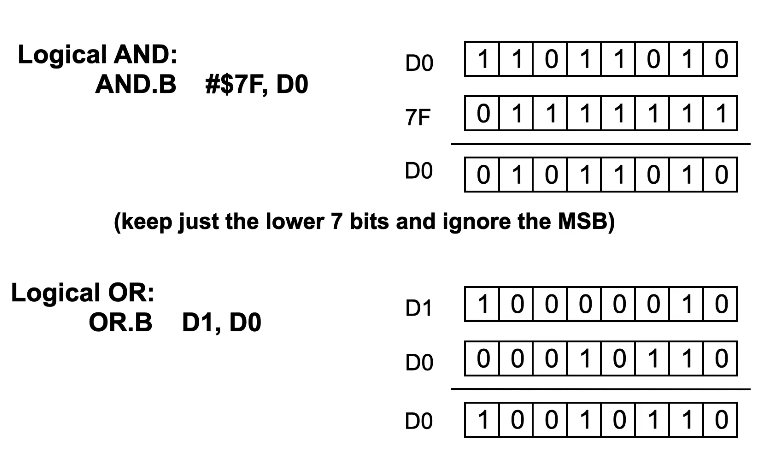
\includegraphics[width=0.8\textwidth]{figures/logicalinst.png}
	\caption{Logical Instructions}
	\label{fig:figures-logicalinst-png}
\end{figure}
Similarly, shifts work by transferring the bits to the left or right. We can do this by multiplying by 2. 
\begin{figure}[H]
	\centering
	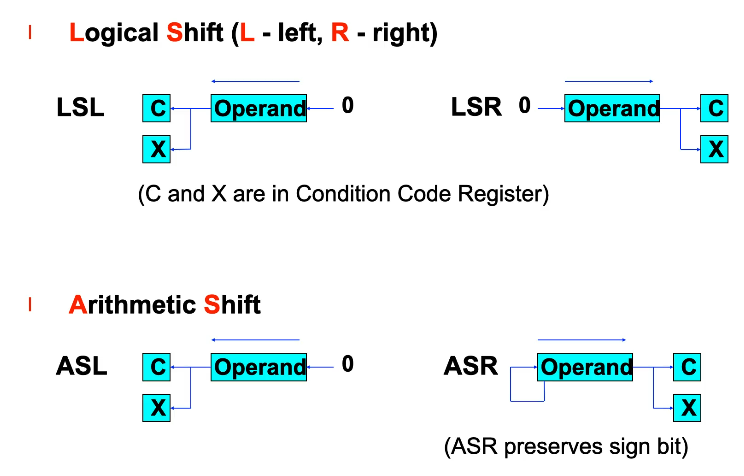
\includegraphics[width=0.5\textwidth]{figures/logic1.png}
	\caption{Shifts left and right}
	\label{fig:figures-logic1-png}
\end{figure}
\begin{figure}[H]
	\centering
	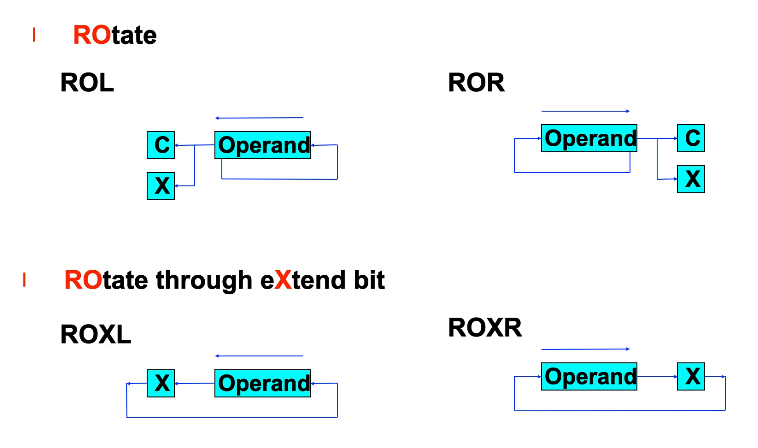
\includegraphics[width=0.5\textwidth]{figures/logic2.png}
	\caption{No fucking clue}
	\label{fig:figures-logic2-png}
\end{figure}
\subsubsection{Subroutines}
Subroutines are useful for frequently used sections of a program.
Write and debug a subroutine once, and use that program code whenever it is needed. It reduces program size and improves readability. The commands are $JSR <label>$ which is jump to subroutine and $RTS$ return from subroutine.
\subsubsection{Stacks}
A stack can be used to capture the last in first out (LIFO) aspect of the assumption we were making. The use of stacks for subroutine calls is common. The JSR pushes the contents of the PC on the stack. Puts start address of subroutine in PC. The return from Subroutine pops the return address from the stack and puts it in PC, so the stack where to from a subroutine.

\subsubsection{Addressing Modes}
How we tell the computer where to find data it needs. It requires to organise application data. Some data never changes, some is variable and some needs to be located within a data structure, e.g. list, table or array.
In $68008$ systems data can be located in data register, within the instructor itself or in external memory.
\begin{tcolorbox}[colback=black!3!white,colframe=black!60!white,title=\begin{exmp}Example \label{Example}\end{exmp}]
        "Heres $100 \$ $" This is a literal value. \\
	"Get the cash from Rootes room $19$" This is absolute address.\\
	"Go to Rootes room 23 and they'll tell you where to get the cash" This is indirect address \\ 
	"Go to rootes room 42 and get the cash from the fifth room to the right" This is relative address.
\end{tcolorbox}
\begin{enumerate}
	\item Data or Address Register Direct - the address of an operand is specified by either a data register or an address register e.g. move  D3, D2
	\item Immediate Addressing - The operand forms part of the instruction and remains constant throughout the execution of a programme. E.g. move.b #\$42, D5 
	\item Absolute Addressing - The operand specified the location in memory explicitly, meaning no further processing required. E.g. move.l D2,\$7FFF0
	\item Relative Addressing - Code like this contains no absolute addresses, i.e. it uses only addresses relative to the current program counter, and therefore can be placed anywhere in memory.
\end{enumerate}
\section{Memory Systems}
\subsection{Memory Hierarchy}
To construct a memory system, we must think carefully about the properties of each storage approach. Many factors include the choice of memory technology such as:
\begin{itemize}
	\item Frequency of access
	\item Access time
	\item Capacity required
	\item Cost e.g. cost per bit
\end{itemize}
\subsubsection{Designer's Dilemma}
The desire for low cost and high capacity - leads to choice of cheap per bit, high capacity and slow access time
Desire high performance - leads to choice of expensive per bit, low capacity and fast access time
In order to solve this problem, we have to choose both by organising memory into a hierarchy.
This leads to the memory hierarchy:
\begin{figure}[H]
	\centering
	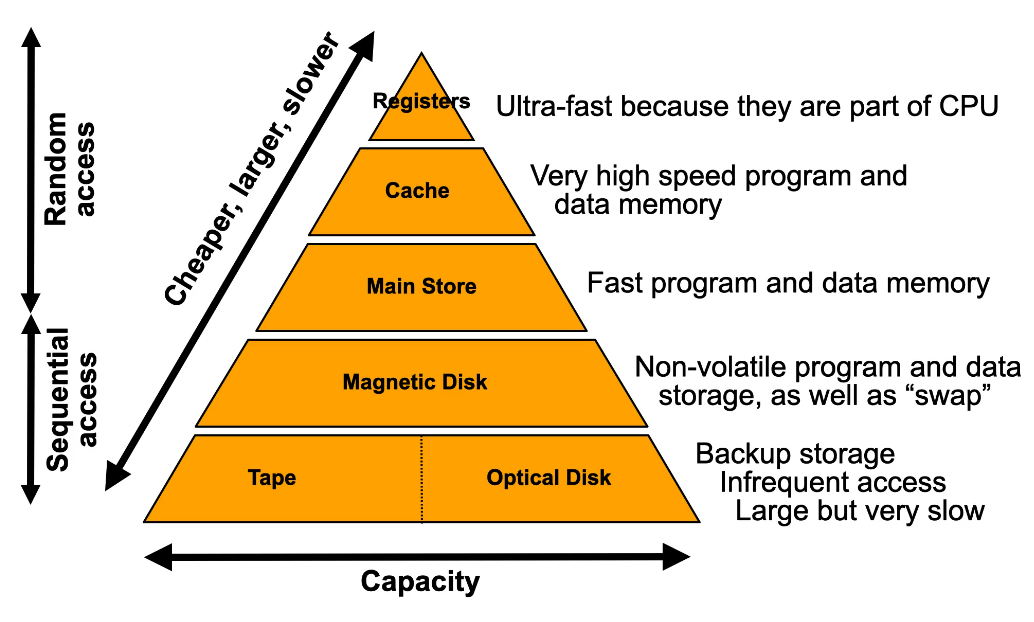
\includegraphics[width=0.8\textwidth]{figures/hierarchy.png}
	\caption{The Memory Hierarchy}
	\label{fig:Hierarchy}
\end{figure}
The reason we have such a hierarchy is indeed because of economics. 
\begin{tcolorbox}[colback=black!3!white,colframe=black!60!white,title=\begin{defn}Temporal Locality \label{Temporal Locality}\end{defn}]
If a particular memory location is referenced, it is likely that the same location will be referenced again in the near feature
\end{tcolorbox}
\begin{tcolorbox}[colback=black!3!white,colframe=black!60!white,title=\begin{defn}Spatial Locality \label{Spatial Locality}\end{defn}]
If a particular memory location is referenced, it is likely that nearby memory locations will be referenced in the near future
\end{tcolorbox}
A reasonable assumption is that it has been shown that $90 \%$ of memory accesses are within $\pm 2$ kilobytes of previous PC position.
\subsection{Semiconductor Memory Types}
\begin{table}[H]
	\centering
	\caption{Semiconductor Memory Types}
	\label{tab:semiconductor}
	\begin{tabular}{c|c|c|c|c}
	Memory Type & Category & Erasure & Write Mechanism & Volatility \\
	\hline
	Random Access Memory (RAM) & Read-write & Electrically at byte-level & Electrically written & Volatile \\
	Read-only Memory (ROM) & Read-only & Not possible & Mask written & Non-volatile \\
	Programmable ROM (PROM) & Read-only & Not Possible & Electrically witten & Non-volatile \\
	Erasable PROM (EPROM) & Read-mostly & UV-light at chip-level & Electrically written & Non-volatile \\
	Electrically Erasable PROM (EEPROM) & Read-mostly & Electrically at byte-level & Electrically written & Non-volatile \\
	Flash Memory & Read-mostly & Electrically at block-level & Electrically written & Non-volatile \\
	\hline
	\end{tabular}
\end{table}
We are particularly interested in random access. Furthermore, RAM is most common type of semiconductor memory, but its title is misleading since all things in the table allow random access.
\subsection{Cache Memory}
Cache is using the term "$90\%$ of memory accesses within only $2$ KBytes"
So store those $2$ KBytes in a small, fast "cache" memory. If data required by CPU is in the cache, it is a huge speed improvement. It is also small to limit cost. It is also possible to have multilevel caches, which there are levels of cache depending on the range of KBytes.
\subsubsection{Concepts}
Cache read-only data is relatively straightforward. We don't need to consider the possibility that items will change, hence copies across memory hierarchy remain consistent. Two general strategies are adopted when caching writes, both of which can employ a buffer to enhance performance
\begin{itemize}
	\item Write Through - update the item in cache and writes through to update lower levels of memory hierarchy
	\item Write Back - only updates copy in cache, ensuring that blocks are copied back to memory when they are replaced
\end{itemize}
\subsubsection{Types of Cache Miss}
Measures of cache performance include hit rate $(h)$ and miss rate $(1-h)$.
\begin{align*}
	h = \frac{\text{Number of times the words are in cache}}{\text{Total number of memory references}}
\end{align*}
We can understand cache misses by sorting all misses into categories:
\begin{itemize}
	\item Compulsory - misses that would occur regardless of cache size e.g. the first access to a block cannot be in cache (regardless of size) so the block must be retrieved
	\item Capacity - misses the occurring because a cache is not large enough to contain all blocks needed during the execution of program
	\item Conflict - misses occurring as a result of the placement strategy for blocks not being fully associative, which means that a block may be discarded or retrieved
	\item Coherency - misses occurring due to cache flushes in multiprocessor systems
\end{itemize}
\subsubsection{Measuring Cache performance}
Performance measures based solely on hit and miss rates don't factor in the cost of a cache miss.
Average memory access time is an alternative measure that accounts for the cost of a cache miss
\begin{align*}
	\text{Average memory access time} = \text{ Hit time } + \text{(Miss rate $\times $ Miss Penalty)}
\end{align*}
This is where hit time is the time to hit in the cache and miss penalty is the time taken to replace the block from the memory. Sometimes, however, this isn't even good enough and execution time can often be a better measure in real-world situations.
\subsubsection{Hierarchy in Cache}
Data storage is a balance of size and speed. Memory is closer to the CPU are the Cache with levels $1$, $2$ and $3$. These are fast but have smaller capacity. Main memory is further and slower but has a far greater capacity and hard disks have the greatest capacity and do not need continuous power, but have the slowest access times. The optimisation then would consist through the use of fastest memory possible for highest performance, but problems may large datasets. The solution, is then, to reuse data already in cache as much as possible and prefetch data from main memory into cache before it is needed, masking load times.
 \subsection{Moore's Law}
"The complexity for minimum component costs has increased at a rate of roughly a factor of two per year. Certainly of the short term this rate can be expected to continue, if not increase. Over the long term, the rate of increase is a bit more uncertain, although there is no reason to believe it will not remain nearly constant for at least $10$ years.". This is not commonly expressed as "The number of transistors on a memory chip doubles every $18$ months".
The effects of this are: 
\begin{itemize}
	\item The cost of computer logic and memory circuitry has fallen at a dramatic rate
	\item As logic and memory is placed closer together on more densely packed chips, the electrical path is shortened, increasing operating speed
	\item Computers have become smaller, making them more convenient for use in a variety of environments
	\item Reduction in power and cooling requirements
	\item Interconnections on an IC are more reliable than solder connections, thus having off-chip connection increases reliability.
\end{itemize}
Unfortunately, as clock speeds and everything else has improved, the memory access speed is improving much more slowly. As such, cache is the core to addressing this challenge.
\subsection{Memory Cell Organisation}
Most common form of main story is the RAM, which break down into two main technologies which are:
\begin{itemize}
	\item Static RAM (SRAM)
	\item Dynamic RAM (DRAM)
\end{itemize}
SRAM uses flip-flop storage element for each bit. \\
DRAM for each bit, uses the presence or absence of charge in a capacitor to denote a $1$ or $0$.
Capacitor charge unfortunately leaks away over time, requires period refreshing, but it is cheaper than SRAM.
\subsubsection{SRAM}
SRAM stores data using configurations of flip-flops and logic gates, and the memory cells hold data as long as there is power supplied. It uses four cross-coupled transistors to establish a stable logic state.
\subsubsection{DRAM}
DRAM memory cells store data as charge on capacitors. Unfortunately, it leads to these issues:
\begin{itemize}
	\item Capacitors naturally discharge, hence DRAM cells require periodic charge to maintain data storage
	\item The term 'dynamic' refers to the natural leakage of charge that takes place even when power is supplied
	\item Presence or absence of charge is interpreted as logical $0$ or $1$
\end{itemize}
We can consider the appreciated the operation of DRAM by considering a $1 $ bit DRAM memory cell.
Address line is activated when the bit value from the cell to be read or written
A transistor acts as a switch that is closed (allowing current flow) if a voltage is applied to the address line and open if a voltage is not applied to the address line (no flow)
\begin{figure}[H]
	\centering
	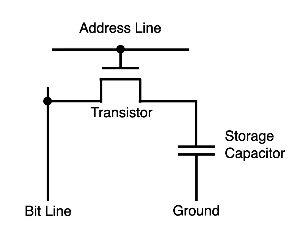
\includegraphics[width=0.4\textwidth]{figures/dram.png}
	\caption{DRAM}
	\label{fig:DRAM}
\end{figure}
The write operations are as follows:
\begin{itemize}
	\item The voltage applied to the bit line which is high for a logical $1$, and low for a logical $0$.
	\item A signal is then applied to the address line, allowing a charge to be transferred to the capacitor (data store)
\end{itemize}
The read operations are as follows:
\begin{itemize}
	\item Transistor turns on when address line is selected, allowing the stored charge to be fed out to the bit line and a sense amplifier
	\item Sense amplifier compared the capacitor voltage to a predetermined threshold value to determine if it is a $0$ or a $1$ 
	\item The read process discharges the capacitor, which means that it must be restored as well as refreshed following the read operation
\end{itemize}
\subsubsection{Comparing DRAM and SRAM}
Both are volatile - power must be continuously supplied
Dynamic memory cells are generally simpler and more compact which allow for greater memory cell density and cheaper to produce than equivalent SRAM memory. \\
Refresh circuitry incurs one-off cost that is only compensated for by larger memory capacities \\
SRAM are typically provide better read and write times than DRAM, meaning that Cache uses mainly SRAM and main memory uses DRAM.
\subsubsection{Organisation of a Memory Chip}
It is critical to maintain a structured approach to the organisation of on-chip memory.
\begin{figure}[H]
	\centering
	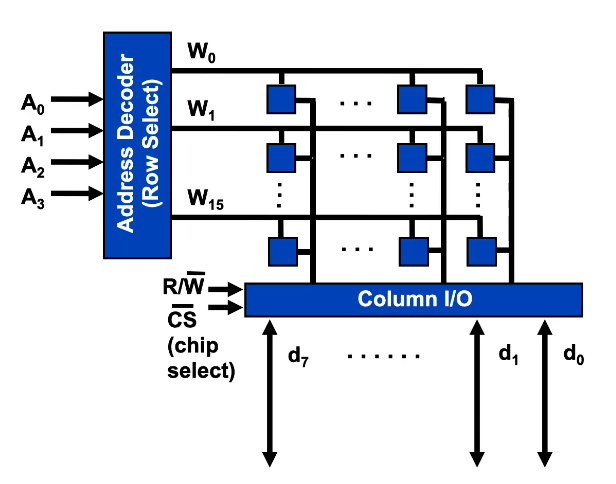
\includegraphics[width=0.5\textwidth]{figures/memorychip.png}
	\caption{$16\times 8$ memory integrated circuit ($16\times 8$ denotes $W\times B$ i.e. words $\times $ bits, each of $8$ bits}
	\label{fig:figures-memorychip-png}
\end{figure}
IC design for $16\times 8 = 128$ cells required $4$ address inputs $= \log_2W$, where $W = \text{no of words}$ and $8$ data lines $B$, where $B = \text{word size}$.
Consider a $1$ KBit $=1024$ cells device. It is possible to organise as a $128\times 8$ memory cell array, requiring $7$ address pins $\log_2 128$ and $8$ data pins, which is a total of $15$ input output pins, plus power etc. Thus, we could take different approaches, but what would be the best way? A $1024\times 1$ would require $10$ address pins and $1 $ data pin, a total $11$ IOs etc. isn't as efficient. The goal is to minimise decoding space. This could be done by dividing the address inputs into $2$ parts - row address and column address. It is then most efficient to have it as a square.
\subsection{Error Detection and Correction}
Error occurs within a computer system, e.g. in system memory, and in the communication between systems, e.g. in the transmission of messages. \\
Noise is unwanted information that can cause these errors. It comes in various forms, but is always present and is one of the limiting factors in computer systems. It can occur from stuff such as thermal noise, noise of electronic components, noise of transmission etc.
\subsubsection{Detecting single and isolated errors}
These are considered to occur at random, usually due to noise. We could send the message three times and take a vote, but this is very expensive. However, if the probability of an error in the channel is low, the probability of two errors close together is also lower. Thus, we can add a "parity" bit to the message every so often, which "summarises" a property of the message that we can check to determine whether a message has been altered. It is much cheaper and adequate in many situations.
\subsubsection{Parity}
Parity adds an extra bit. There are two types of parity system:
\begin{itemize}
	\item Even parity system - the value of the extra bit is chosen to make the total of logic $1$ an even number
	\item Odd parity system - Make the total number of logic $1$ s odd
\end{itemize}
And it is very popular in hardware. In fact, hardware implementations generally work better than software, despite being a relatively simple digital logic circuit. \\

To detect error using parity, consider our transmitter encoding a $7$ bit message, then, we compute parity $P$ and append parity to message, and send modified message across channel. Now that we receive the message, an $8$ bit is received including parity is decoded. We compute parity $Q$ form data bits of received message and compare our parity $Q$ to parity $P$ in message and flag \textit{ERROR} if they are not consistent. However, if we have say, an odd or an even number of errors depending on the parity, the system does not work very well. These are called Burst Errors. 
\subsubsection{Burst Error}
When the parity is the same but it is still not the same message that was sent, we can create burst error checkers as well. One way to do so is using checksum. For example, we send the word "MESSAGE", which is $1001101, 1100101, 1110011,1110011,1100001,1100111,1100101$. So we calculate the bit-column parity "checksum" values, e.g. using even purity to get
 \begin{align*}
	1001011 = \text{ASCII "K"}
\end{align*}
Then we send "MessageK" instead of "Message". This detects all burst errors $<14$ bits. However, it does fail if an even number of errors occur in a bit-column. What we can do instead, is not just also calculate the bit-column parity, but also calculate the bit-row parity. This is called the ECC. This way, we can identify if a column is wrong when received. Furthermore, we can also detect if a row is wrong, and as such, we can detect which character is exactly wrong and correct it.
\subsection{Common Memory Components}
\subsubsection{Hard Disks}
Record data by magnetising a thin film of ferromagnetic material on a disk. As well as its operations, the general structure of a hard disk can give us insight into performance issues. In terms of data organisation, one track contains many sectors, which each sector being separated by an inter-sector gap. Sector contains preamble to allow head to be synchronised before read/write, data and ECC. The performance of hard disks isn't that great.
\subsubsection{Optical Disks}
Originally designed to hold music, spiral is $3.5$ miles long if unwound and data encoded as "pits" and "lands". Errors in an optical disk are usually local because of scratches, if they're less than $2$ mm, it can be corrected. The performance is very good, seek times averages are typically $80$ ms.
\section{I/O Systems}
\subsection{Memory Mapped I/O}
The same address bus is used to address both memory and I/O devices. Memory, including register, on I/O devices are mapped to address values. An I/O device can then operate as designed on the data given. When a CPU accesses a memory address, that memory address may be in physical memory (typically RAM) or be associated with memory of an I/O device. The advantages of a memory-mapped I/O are following:
\begin{itemize}
	\item Simpler than many alternatives (compared to port I/O where a dedicated class of instructions are set)
	\item CPU requires less internal logic as a result, making it cheaper
	\item All addressing modes supported by a CPU are available to I/O
\end{itemize}
And the disadvantages:
\begin{itemize}
	\item Portions of memory address space must be reserved
	\item Less of a concern as $64$ bit processors, hence address spaces, have come to market
	\item Still relevant where $16$ bit and sometimes $32$ bit processors are used e.g. embedded and legacy systems
\end{itemize}
\subsection{Synchronising with I/O devices - Polling}
Most I/O devices are much slower than the CPU. Several issues to consider:
\begin{itemize}
	\item Read - is there data to be read from the device?
	\item Write - is the device ready to accept data?
\end{itemize}
Consider a simple printer that takes a finite amount of time to print a character. It is much faster than processor instruction time
\subsubsection{Polling and Busy-wait Polling}
\begin{figure}[H]
	\centering
	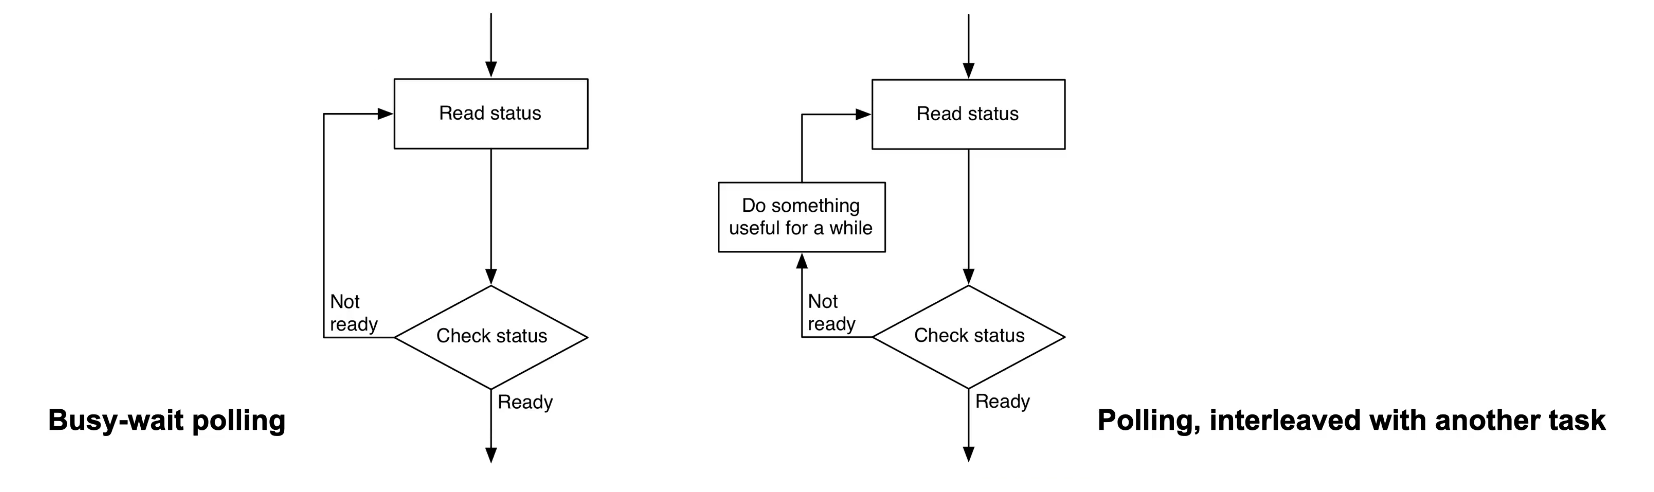
\includegraphics[width=1\textwidth]{figures/polling.png}
	\caption{Polling}
	\label{fig:polling}
\end{figure}
\subsubsection{Advantages}
\begin{itemize}
	\item Simple software - a looping construct paired with some known checks
	\item Simple hardware - support for notion of "ready" is all that is required
\end{itemize}
\subsubsection{Disadvantaging}
\begin{itemize}
	\item Busy-wait polling wastes CPU time and consumes power
	\item Polling when interleaved with other tasks can lead to significantly delayed response to device
\end{itemize}
\subsection{Synchronising with I/O devices - Handshaking}
\subsubsection{Unsynchronised}
Computer system transfers the data to the output device
\subsubsection{Open-ended handshaking}
The computer system provides data and then assert its validity to the IO device. It is then the device's responsibility to use the data as it fits
\subsubsection{Closed-loop handshaking}
The recipient asserts readiness to receive. The computer system gives and validates the data. The point is that it establishes a period of time that is known to both parties.
\subsubsection{Timing Diagram}
The computer system responds to the printer being ready by placing a new character on the data bus and signalling DATA\_VALID. We would write code to get the CPU to do this, or alternatively, we could use specialised hardware, which often requires fewer CPU instructions.
\begin{figure}[H]
	\centering
	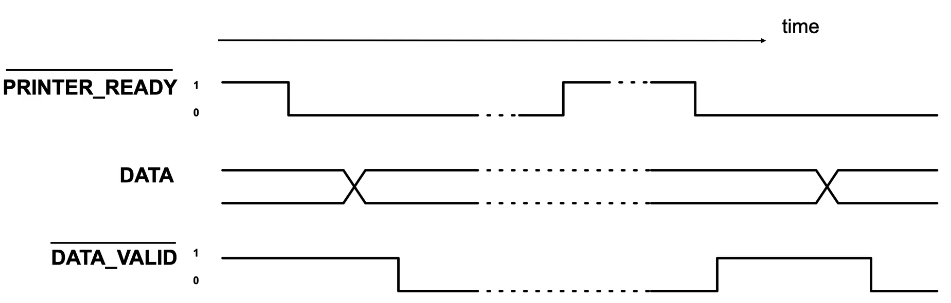
\includegraphics[width=0.65\textwidth]{figures/timing.png}
	\caption{Timing Diagram}
	\label{fig:timing}
\end{figure}
\subsection{Synchronising with I/O devices - Interrupts}
Consider the $6502$ processor, designed in $1975$, used in the BBC micro and others. IRQ (Interrupt requested) and NMI (Non-maskable interrupt) inputs. Code can disable response to IRQ, as it is only a request, but NMI cannot be disabled or "masked out". 
\subsubsection{Effect of an interrupt input}
CPU normally executes instructions sequentially, unless a jump or branch is made. An interrupt input can force CPU to jump to a service routine. It can therefore make it appear that the CPU is performing two or more tasks simultaneously" 
\subsubsection{Interrupt Handling Sequence}
\begin{enumerate}
	\item External device signals interrupt
\end{enumerate}
INTERRUPT RESPONSE
\begin{enumerate}
	\item CPU completes current instruction
	\item Push PC onto Stack
	\item Push status register(s) onto stack
	\item Load PC with address of Interrupt Handler
\end{enumerate}
RETURN FROM INTERRUPT
\begin{enumerate}
	\item Pop PC from Stack
	\item Pop Status Registers from Stack
	\item Load PC with popped return address
\end{enumerate}
\subsubsection{Nested Interrupts}
\begin{figure}[H]
	\centering
	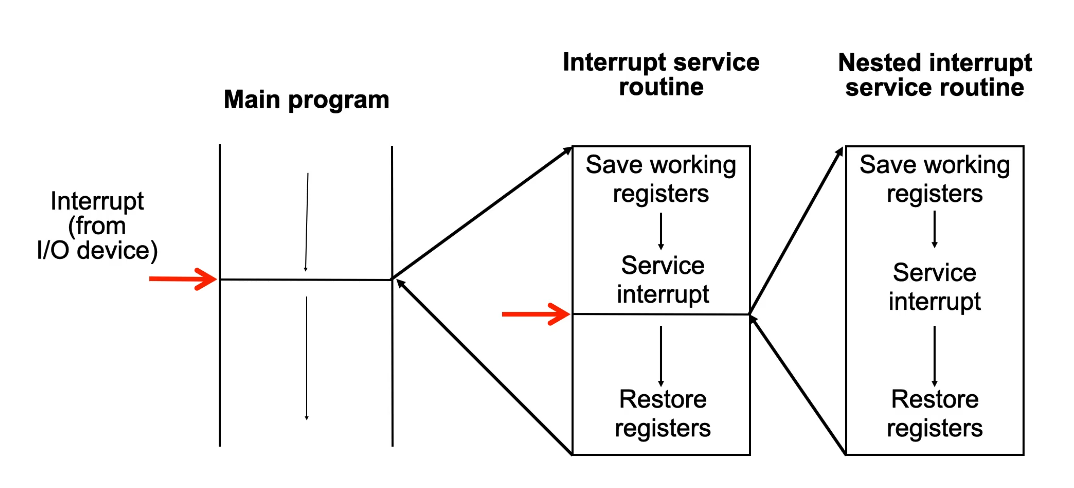
\includegraphics[width=0.8\textwidth]{figures/nestedinterrupt.png}
	\caption{Nested Interrupt}
	\label{fig:nestedInterrupt}
\end{figure}
\subsubsection{Interrupts for I/O Examples}
Switches can be connected to IRQ, if using switches we can OR them all together to form IRQ and then check the individual switch states within the service routine \\
A hard drive can generate an interrupt when data, requested some time earlier, is ready to read \\
A timer can generate an interrupt every 100ms and the service routine can then read a sensor input \\
A printer can generate an interrupt when it is ready to receive the next character to print, as we will see
\subsubsection{Advantages of Interrupts}
\begin{itemize}
	\item Fast response
	\item No wasted CPU time / battery power
\end{itemize}
\subsubsection{Disadvantages of Interrupts}
\begin{itemize}
	\item All data transfers still controlled by CPU
	\item More complex hardware and software
\end{itemize}
\subsection{Direct Memory Access (DMA)}
The CPU is a bottleneck for the I/O. Programmed I/O techniques, as in all the examples, we've seen so far, are slowed down by CPU. \\
DMA is used where large amounts of data must be transferred at high speed. Control of the system buses is surrendered by the CPU to a DMA Controller (DMAC).
\begin{itemize}
	\item The DMAC is a dedicated device that controls the three system buses during a data transfer
	\item The DMAC is optimised for one operation i.e. data transfer
	\item The CPU is more general purpose, it both transfers data and is a processor of information.
\end{itemize}
DMA-based I/O can be more than 10 times faster than CPU-driven I/O
\subsubsection{DMA Operation}
\begin{enumerate}
	\item DMA transfer requested by I/O
	\item DMAC passes request to CPU
	\item CPU initialises DMAC and then requires the following information:
		\begin{enumerate}
			\item Input or Output
			\item Start Address $\to $ DMAC Address Reg.
			\item Number of words transfer $\to $ Count Reg.
			\item CPU enables DMAC
		\end{enumerate}
	\item DMAC requests use of system buses
	\item CPU responds with DMA Ack when it's ready to surrender buses
\end{enumerate}
\subsubsection{Modes of Operation}
\begin{itemize}
	\item Cycle stealing - the DMAC uses the system buses when they are no being used by the CPU - usually by "grabbing" available memory access cycles not used by the CPU
	\item Burst mode - DMAC requires system buses for extended transfer of large amounts of data at high speed and "locks" the slower CPU out of using the system buses for a fixed time or until the transfer is complete or the CPU receives an interrupt from device of greater priority
\end{itemize}
\section{Processor Architecture}
\subsection{Microprocessor Organisation}
\subsubsection{Mainstore and Instructions}
\begin{figure}[H]
	\centering
	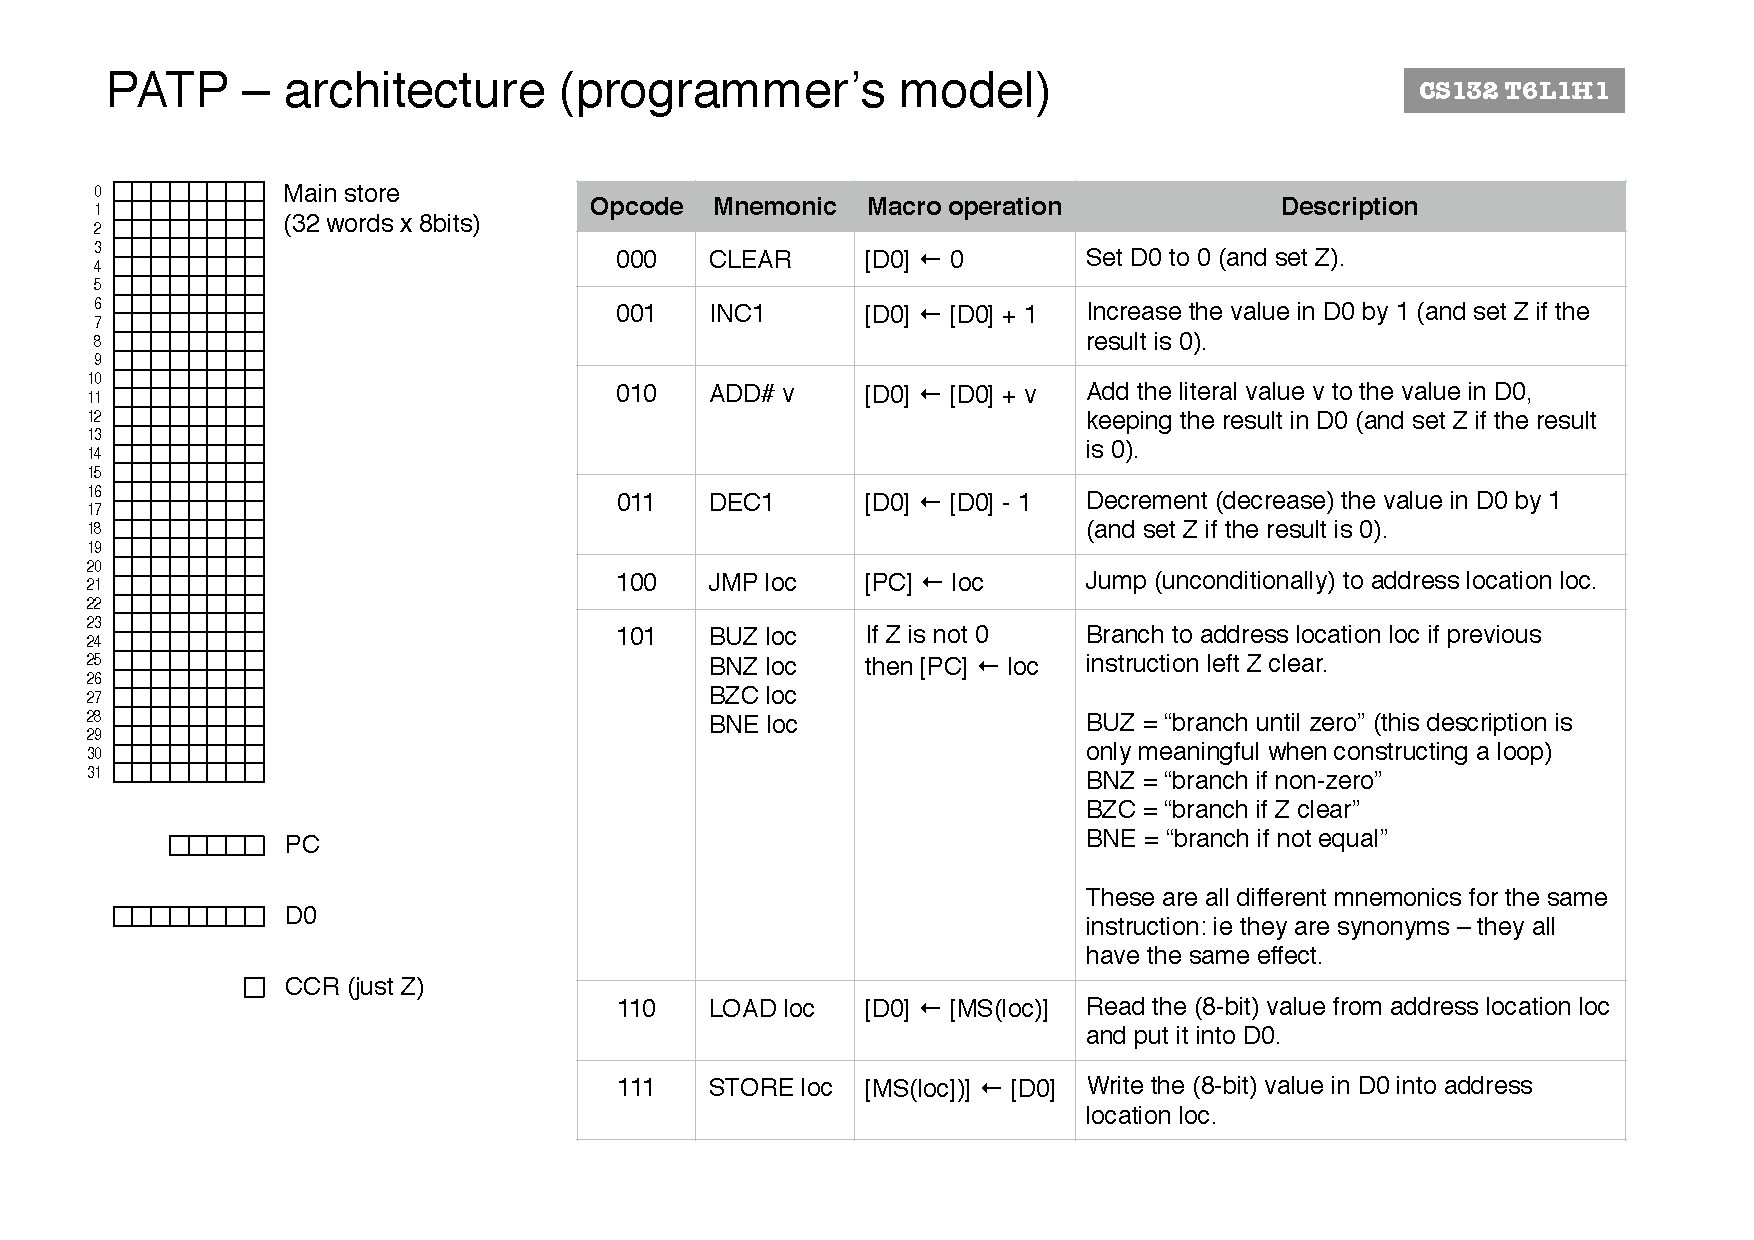
\includegraphics[width=1\textwidth]{PATP/1.pdf}
	\caption{Handout $1$ }
\end{figure}
\subsubsection{Register}
The register is shown as
\begin{figure}[H]
	\centering
	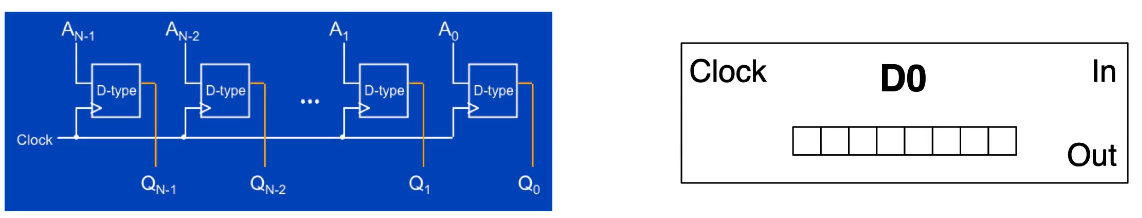
\includegraphics[width=0.8\textwidth]{figures/register2.png}
	\caption{Register}
	\label{fig:register2}
\end{figure}
And will be used for $D 0$, the only data register in our processor
\subsubsection{Arithmetic Logic Unit}
\begin{figure}[H]
	\centering
	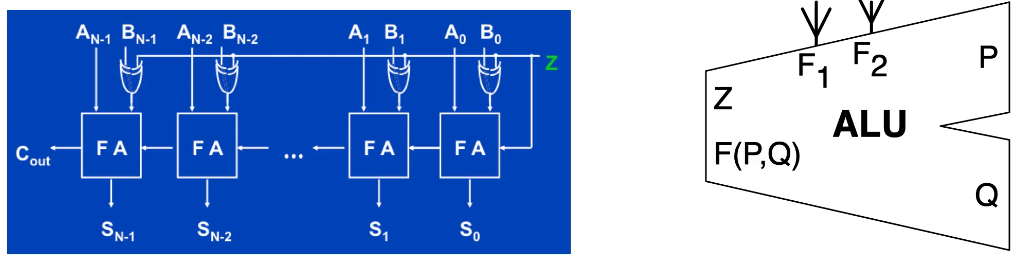
\includegraphics[width=0.8\textwidth]{figures/alu.png}
	\caption{Arithmetic Logic Unit}
	\label{fig:figures-alu-png}
\end{figure}
The arithmetic logic unit ALU is shown above. The inputs are $P$ and $Q$. Sometimes, we want the condition register $Z$. The $F_1$ and $F_2$ are function select and show us what functions we will be computing given $P$ and $Q$.
\subsubsection{Bus}
We will have a common bus for different subsystems to communicate with each other. Three way logic will enable this. This will be done using the enable signals that will be under control of the control unit.
\subsubsection{Control Unit}
Control unit has been largely a black box until now. However, this is the part that regulates the Fetch Decode Execute system and requires to approach the clock speed of the microprocessor. Furthermore, it requires to know the state of the microprocessor and thus requires to know the $Z$ flag. It also takes opcode as input and asserts the set of signals e.g. R/W. 
\begin{figure}[H]
	\centering
	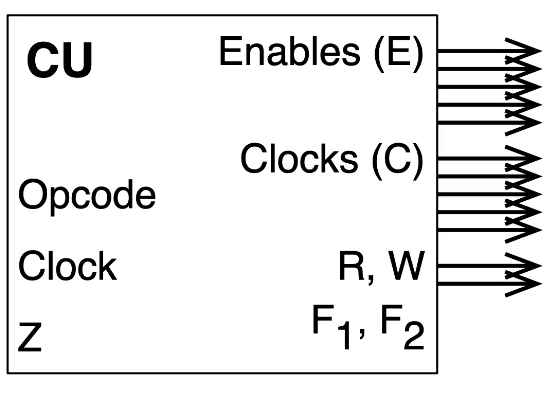
\includegraphics[width=0.3\textwidth]{figures/c.png}
	\caption{Control Unit}
	\label{fig:figures-c-png}
\end{figure}
\subsubsection{Internal Organisation}
\begin{figure}[H]
	\centering
	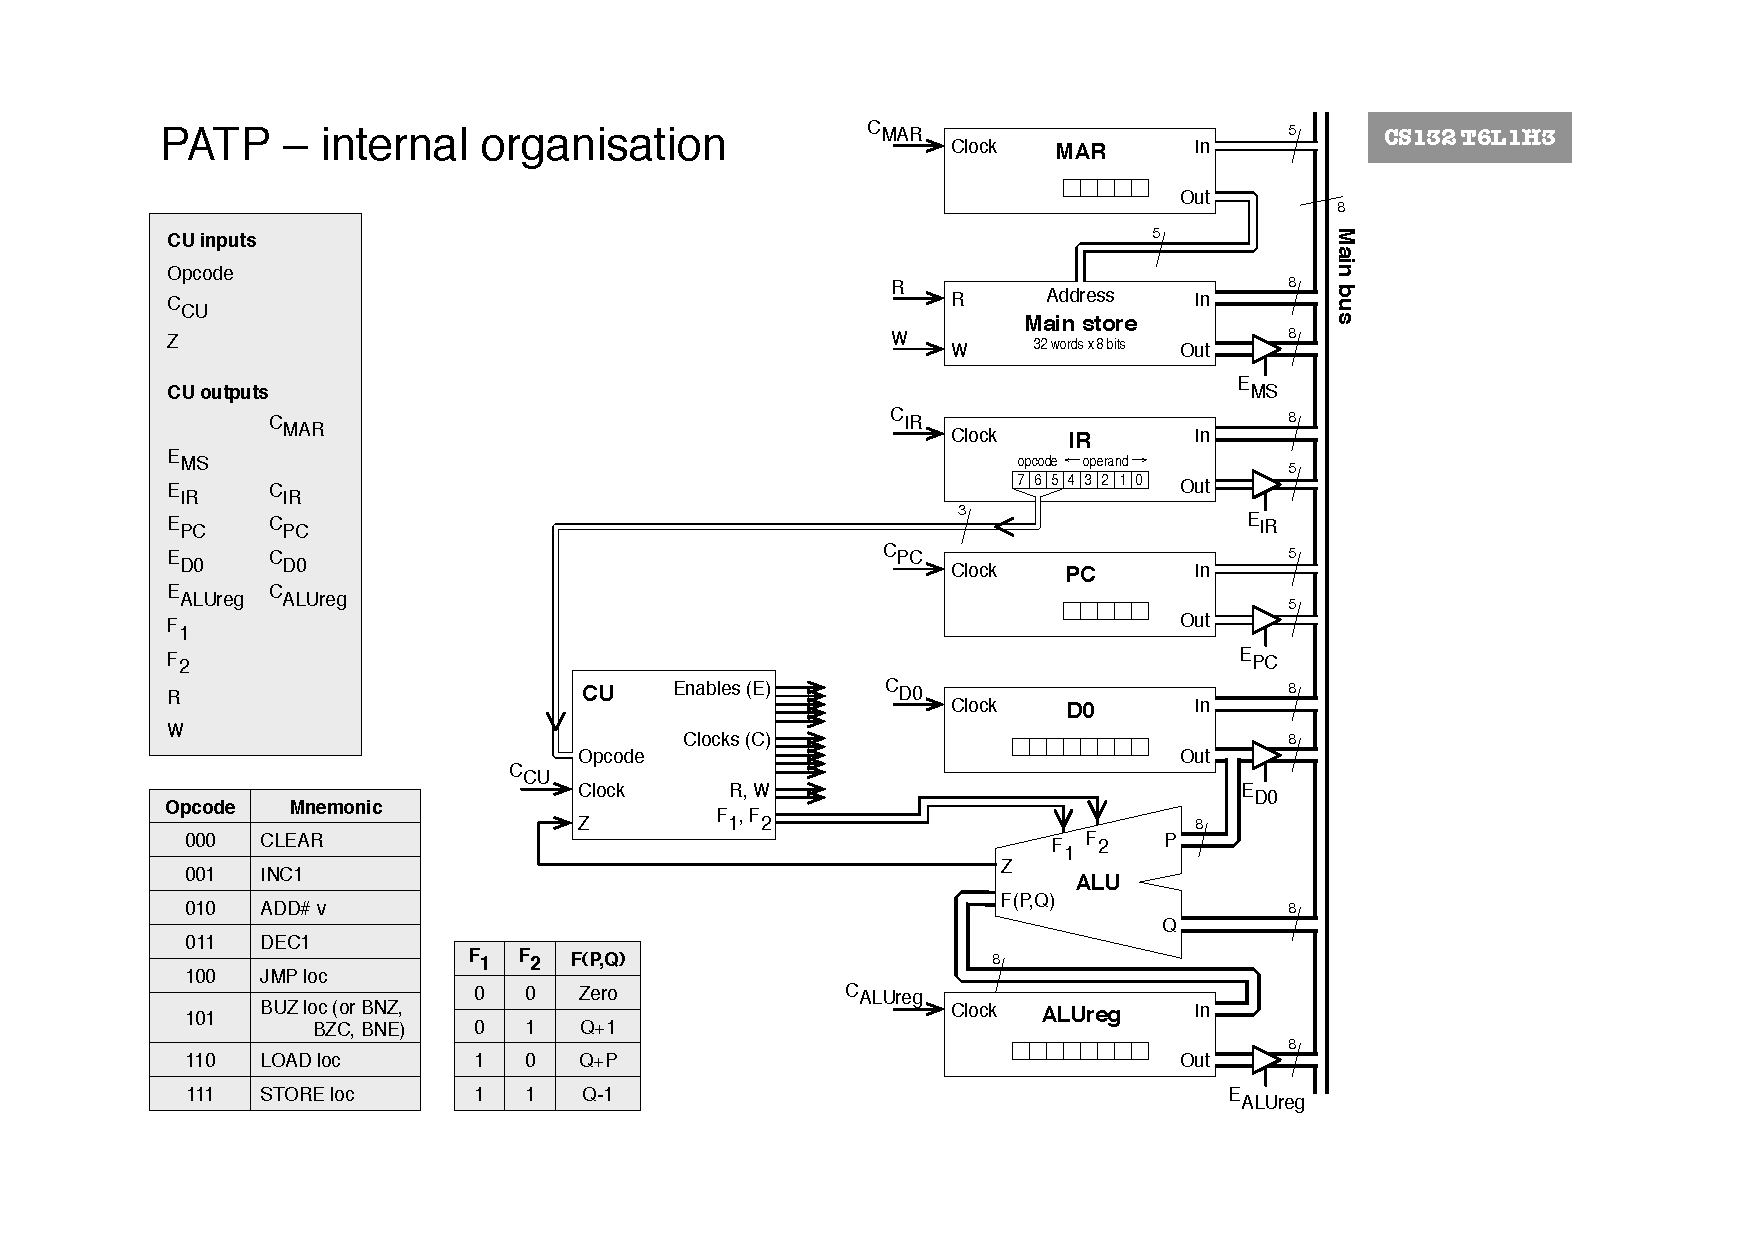
\includegraphics[width=1\textwidth]{PATP/3.pdf}
	\caption{Handout $3$}
	\label{fig:PATP-3-pdf}
\end{figure}
In handout $3$, all these parts come in together to form the PATP, our processor. One thing to note, is that the enable lines, Read, Write etc. are actually connected to the CU, but these connections are not shown because it gets messy quickly otherwise. 
\subsubsection{Instructions and Control Signals}
\begin{figure}[H]
	\centering
	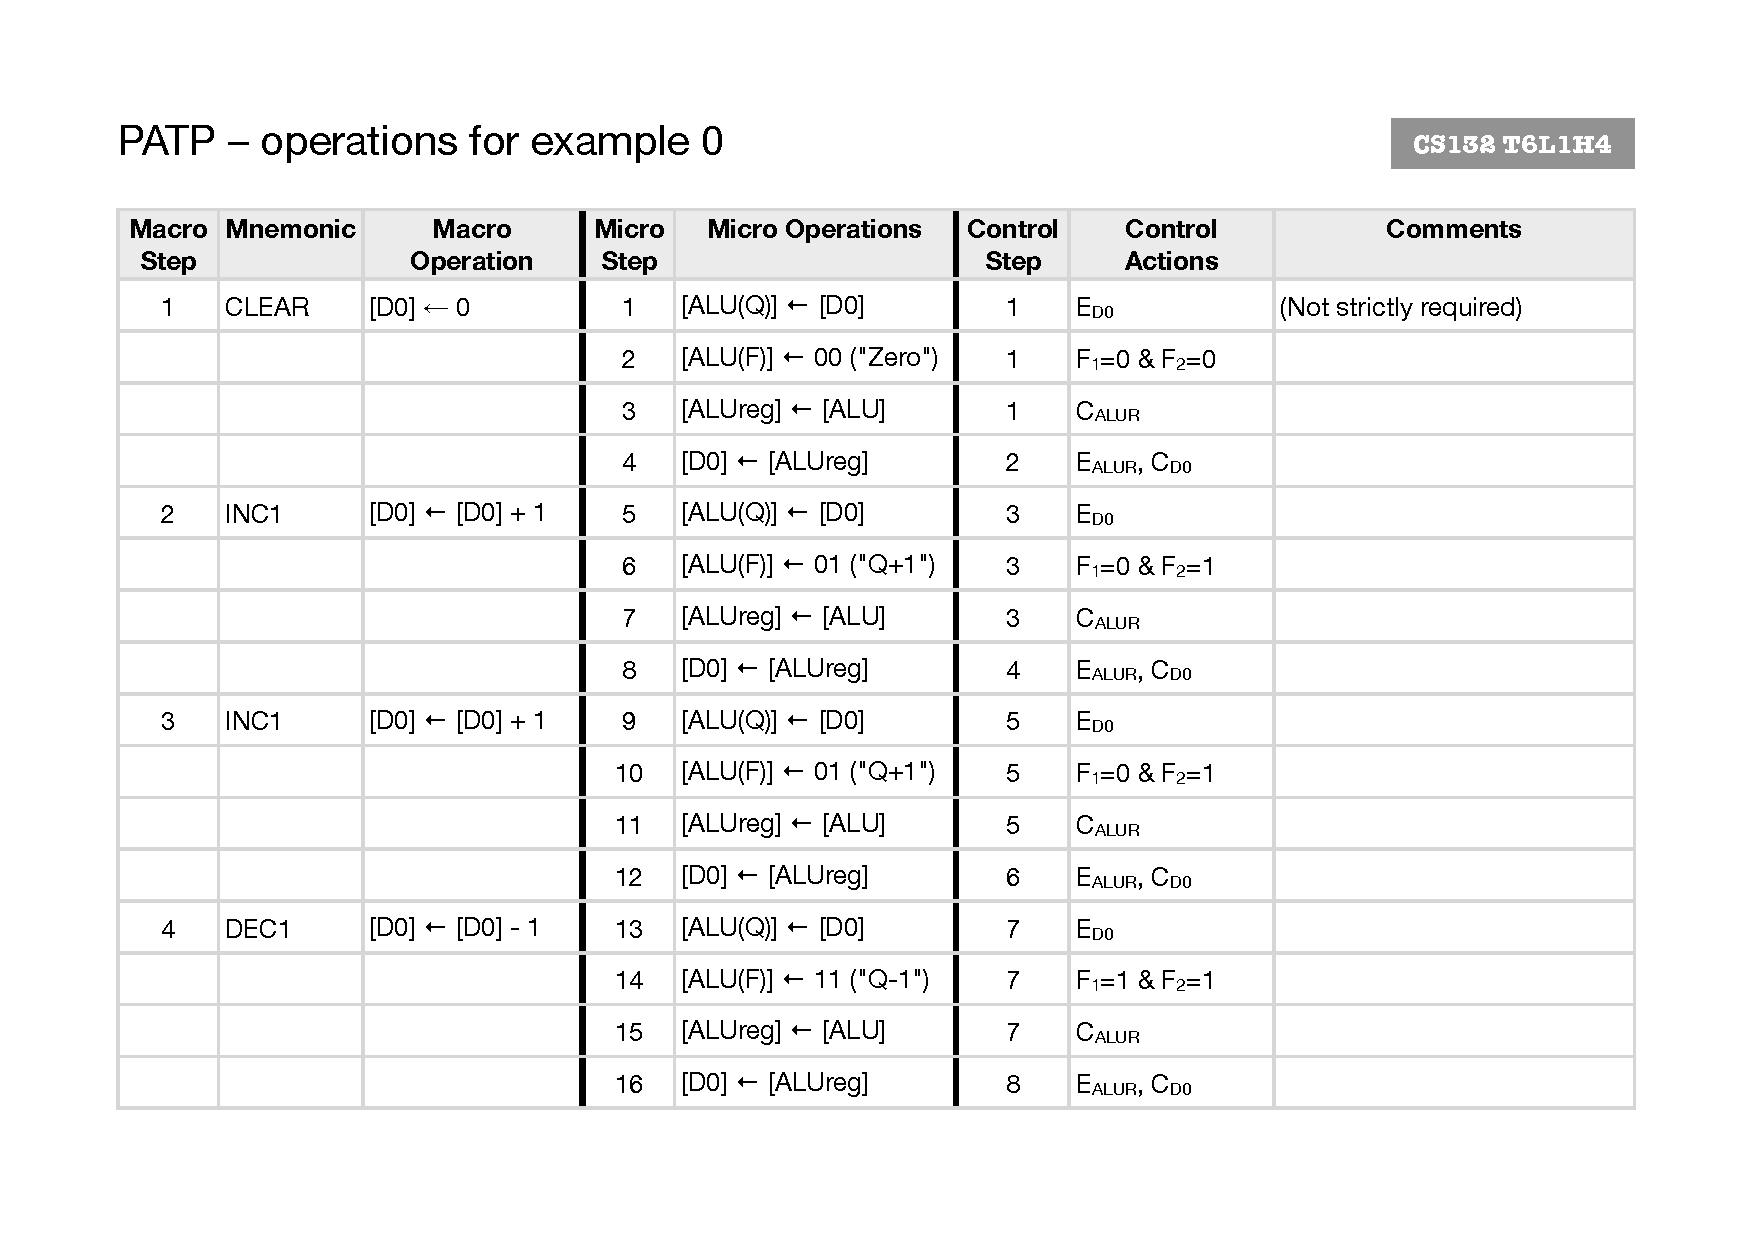
\includegraphics[width=1\textwidth]{PATP/4.pdf}
	\caption{Handout $4$}
	\label{fig:PATP-4-png}
\end{figure}
For example, if we were to have $42$ in binary in $D 0$, the it would first be outed into the bus and into the ALU, then have the correspond $F$ for $Q+ 1$, and then would be stored in $ALUreg$. Then, it would be outputted into the bus and back into $D 0$.
\begin{figure}[H]
	\centering
	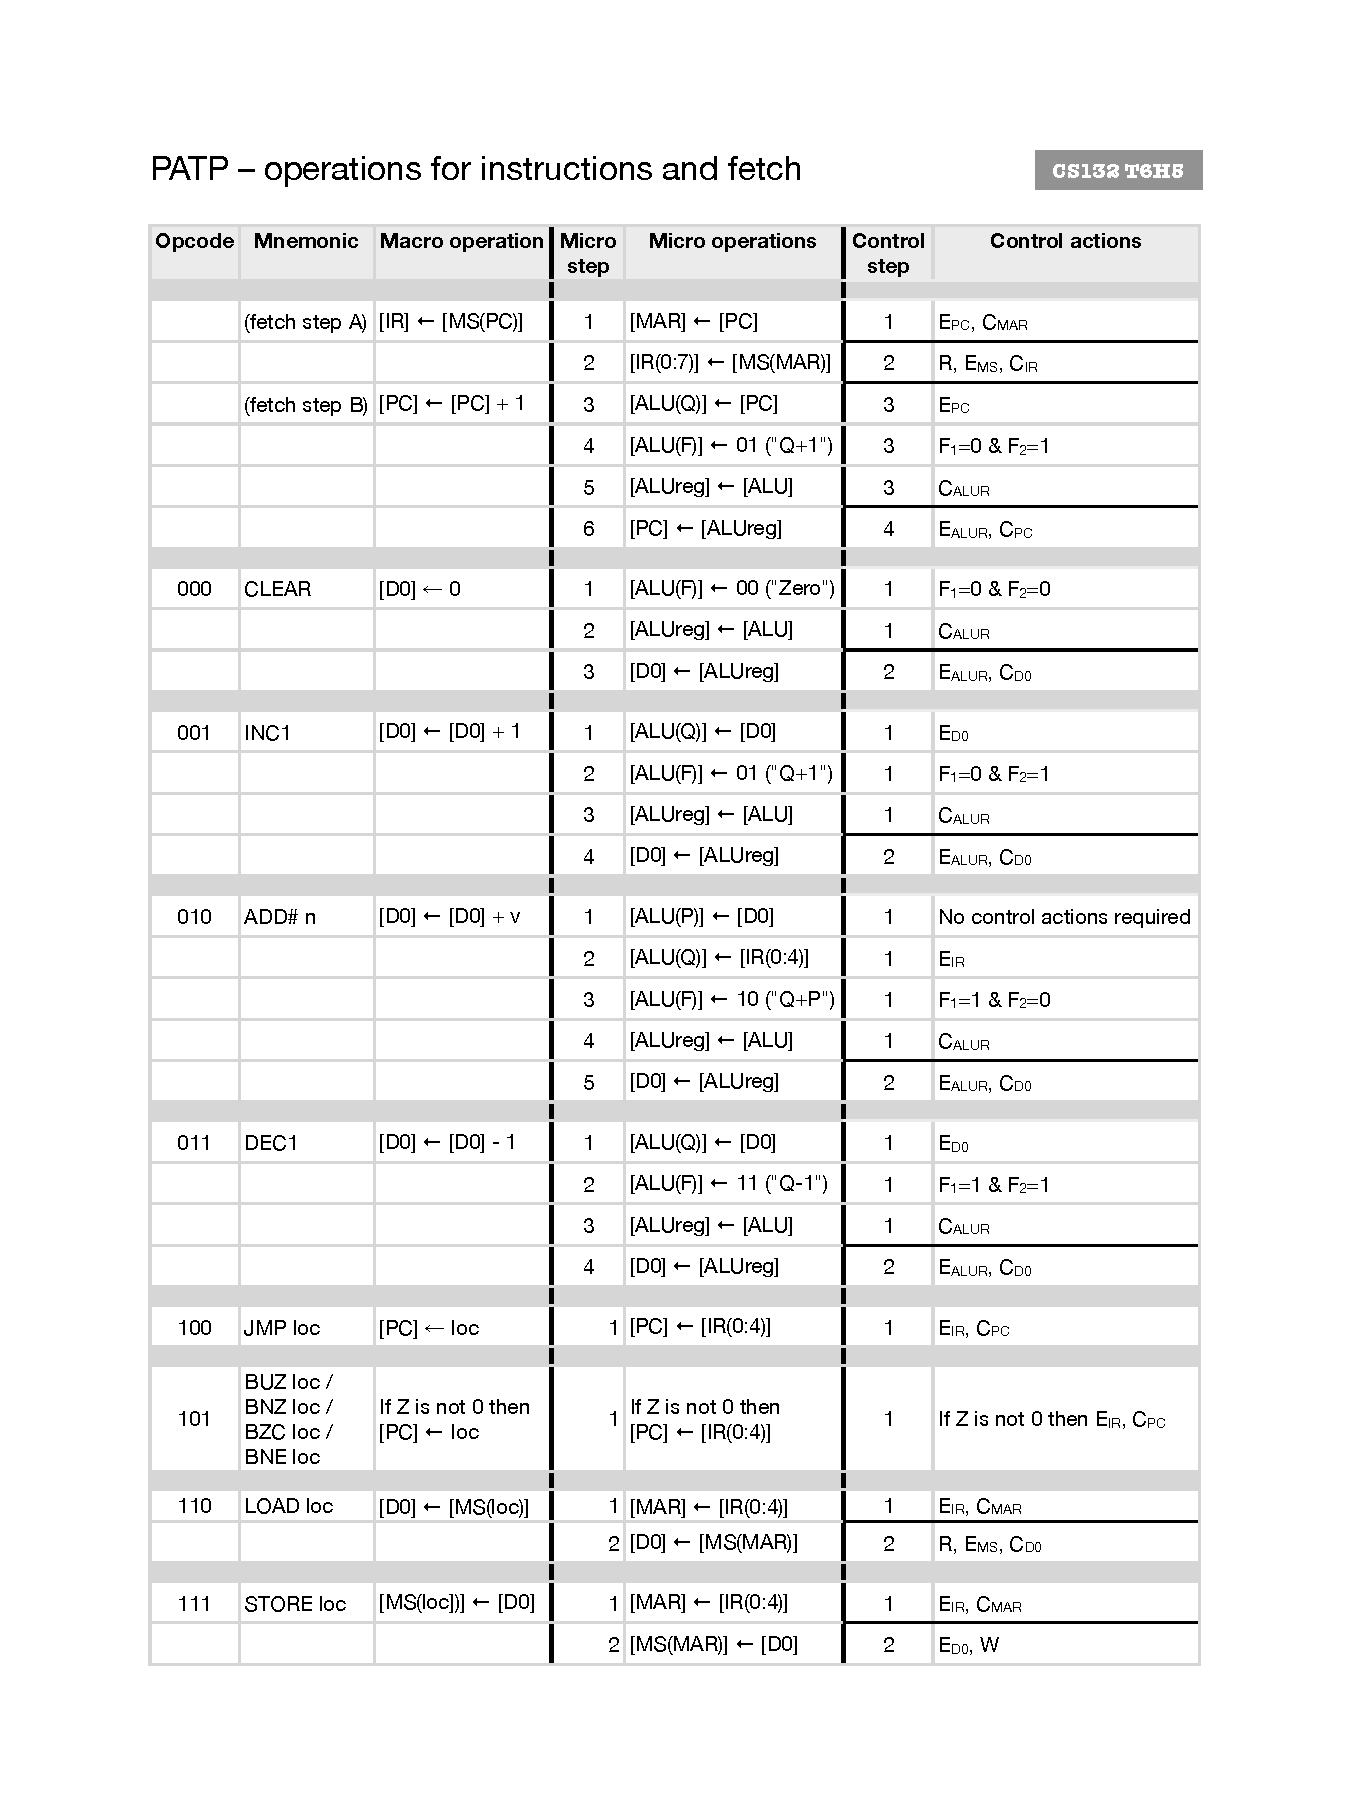
\includegraphics[width=1\textwidth]{PATP/5.pdf}
	\caption{Handout $5$}
	\label{fig:PATP-5-pdf}
\end{figure}

\subsection{Macro and Micro Instructions}
\subsubsection{Fetch Macro Instructions}
The fetch cycle for the PATP would be defined as
\begin{lstlisting}[language = Code]
[IR] <- [MS(PC)] // Get the byte from memory that PC is pointing to, put it in IR
[PC] <- [PC+1] // Increment PC to point to the next byte
\end{lstlisting}
For example, for the program that uses $CLEAR$, $ADD\# 9$ and $DEC 1$:
\begin{figure}[H]
	\centering
	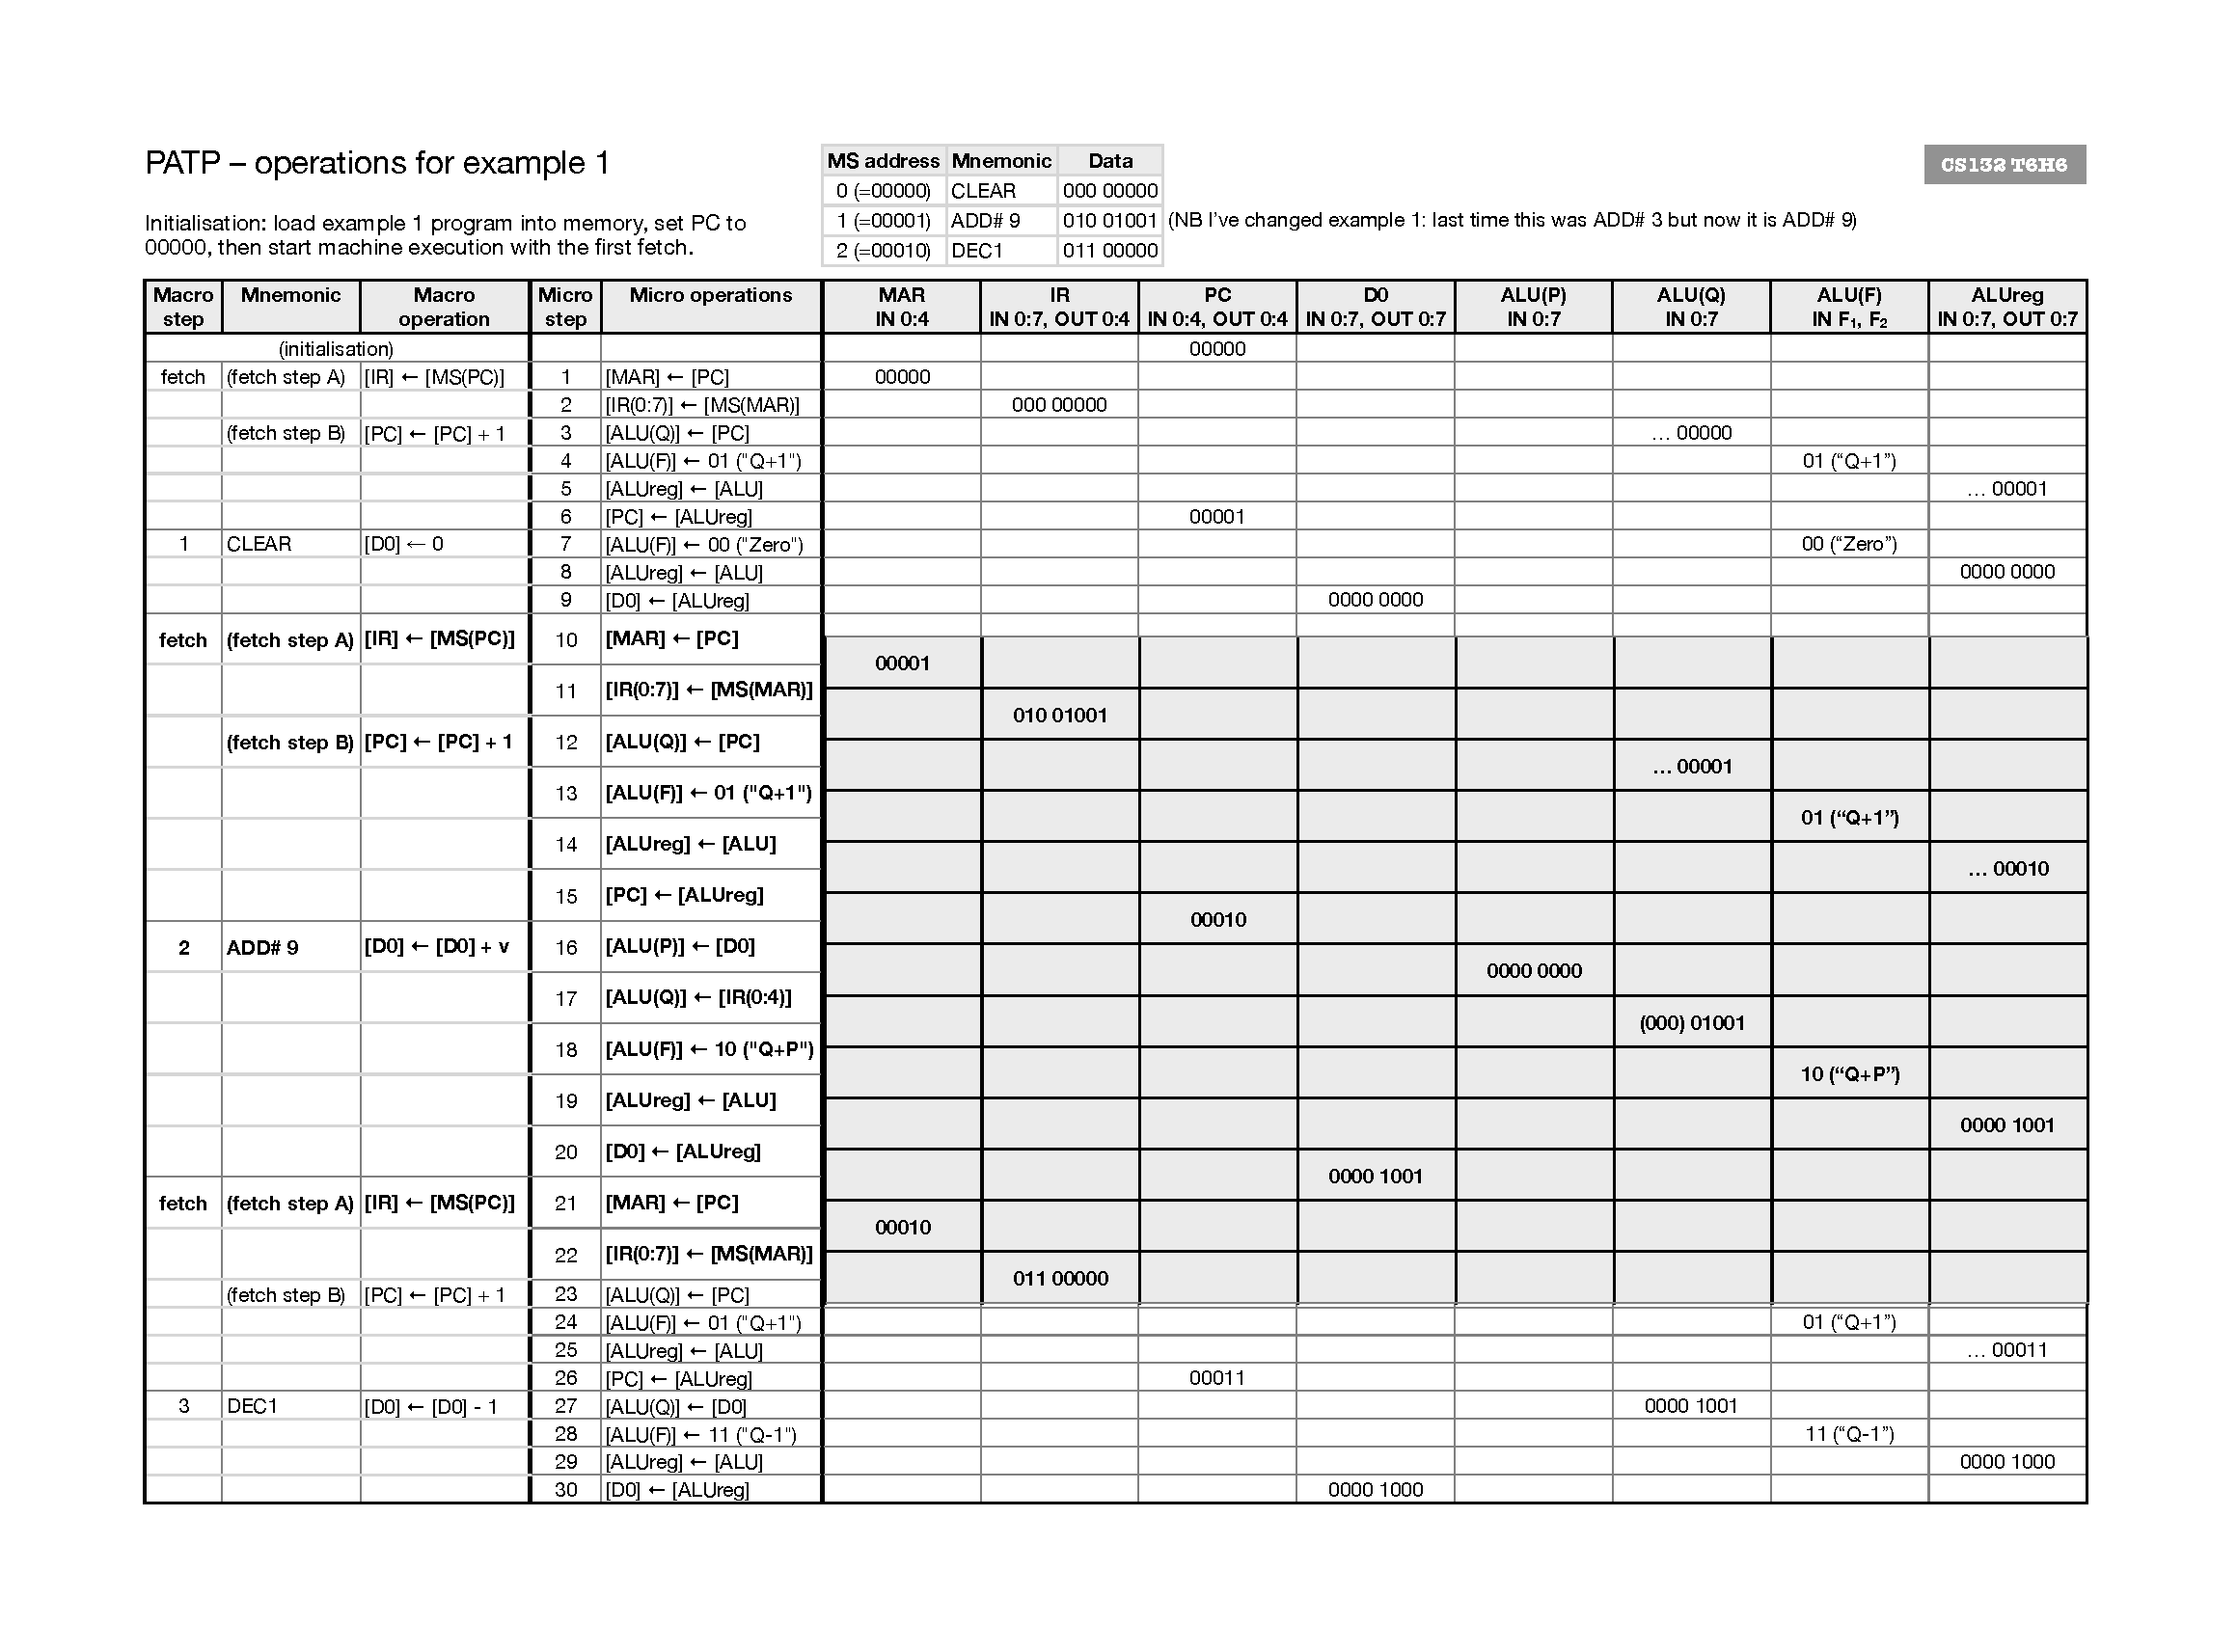
\includegraphics[width=1\textwidth]{PATP/6.pdf}
	\caption{Handout $6$}
	\label{fig:PATP-6-pdf}
\end{figure}
% Question to ask is, where are operands defined or how and what is IR split into two numbers e.g. IR(0:4) and how does it relate to operands
\subsubsection{Assumptions}
\begin{itemize}
	\item Enable signals are level triggered
	\item Clock signals are falling-edge triggered
	\item An output can be enabled onto the main bus and then clocked in elsewhere in one step
\end{itemize}
\subsection{Control Unit Design}
\subsubsection{Control Unit Tasks}
Our goal is to generate fetch control sequence. Observe opcode input and choose the right control signal, that is to decode. And depending upon opcode input, generate sequence of control signals, that is execute. The are two ways to design this:
\begin{itemize}
	\item Hardwired - The CU is combinatorial logic circuit, transforming its input signals into a set of output signals
	\item Microprogrammed - each machine instruction is turned into a sequence of primitive microinstructions, which form a microprogram, stored in ROM called microprogram memory
\end{itemize}
\subsubsection{Hardwired CU}
WE employ the use of a sequencer, that is, we build a logic circuit that produces these outputs if we connect an input to it that repeatedly clocks up and down. In practice, we connect the clock input of the sequencer to CU clock input (CCU)
\begin{figure}[H]
	\centering
	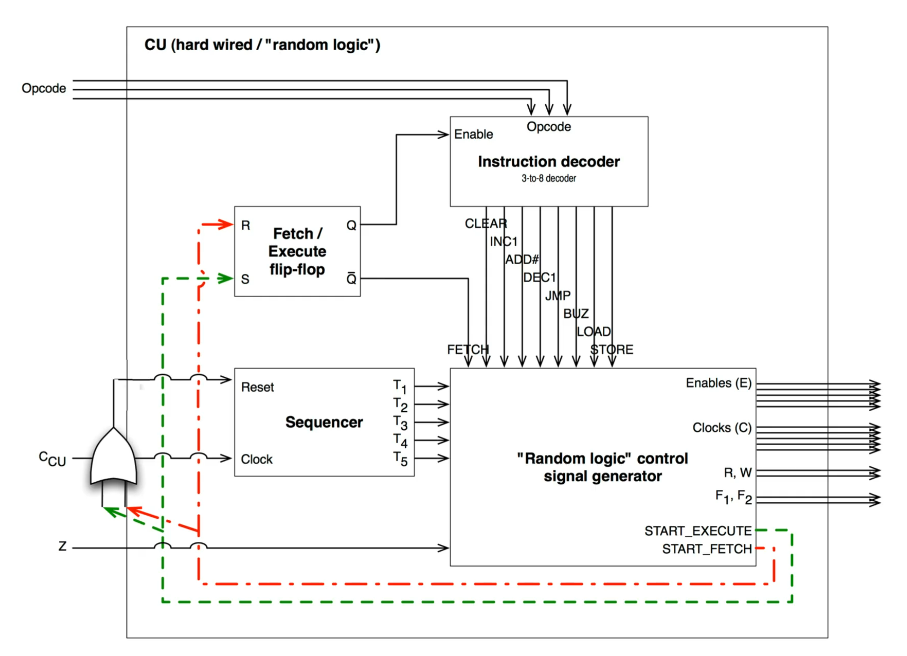
\includegraphics[width=0.8\textwidth]{figures/hardwire.png}
	\caption{Hardwired CPU design}
	\label{fig:figures-hardwire-png}
\end{figure}
The macro instructions go to the random logic control signal generator that determines the outputs. For example, if it recognises if it is the increment operation, we know what enables and clocks require to be on each rounds. The round number is regulated by the sequencer. We will also require a mechanism to move onto the next round, and this is done by the fetch execute flip flop.
\subsubsection{Advantages of Hardwired CU}
\begin{itemize}
	\item It is fast
\end{itemize}
\subsubsection{Disadvantages of Hardwired CU}
\begin{itemize}
	\item Complex hardware makes it difficult to design and test - too many interconnections to get it right
	\item Inflexible as it is difficult to change the design if a new instruction must be added
	\item Long design time
\end{itemize}
\subsubsection{Microprogrammed CU}
This employs the use of a microprogram memory and requires to store the required control action in memory. What we do is we store the round of control signals in each round and look them up as we advance using the microprogram counter. The terminology is as follows:
\begin{itemize}
	\item Microprogram routine - describes how to generate the CU outputs for one macroinstruction 
	\item Microaddress - A location within microprogram memory
	\item MicroPC - The CU's internal program counter, i.e. points to microaddress
	\item MicroIR - The CU's internal microinstruction register is used to hold the current microinstruction
	\item Microinstruction - Holds the CU output values and other fields to control the microprogram flow
\end{itemize}
It is also the dominant technique for implementing CUs for CISC processors
\subsubsection{Advantages of Microprogrammed CU}
\begin{itemize}
	\item Ease of design and implementation
	\item Flexibility of design allows families of processors to be built
	\item Simple hardware compared to hardwired implementation
	\item Microprogram memory can be reprogrammed for new instructions
\end{itemize}
\subsubsection{Disadvantages of Microprogrammed CU}
\begin{itemize}
	\item Slower than hardwired implementations
\end{itemize}
\subsection{How could we change our PATP?}
We could add more memory for more complex applications, we would also need to increase the operand size for things such as branch operations. We could also add more instructions, e.g. subtraction, multiply, divide, and, or operators. This would require a higher upcode size. We could also add more registers and more instructions to these new registers. We could implement floating point, as we are only working with integers. However, the consequences of these improvements is increasing opcode, operand size, increasing complexity etc. \\

The PATP is turing complete, it can complete a universal turing machine and can evaluate every computable function. It can also perform any calculation that any other programmable computer is capable of, however, there are also caveats. These caveats are ignoring time that the machine takes to execute a program, pretending the machine has unlimited storage and addressing and ignoring effort to write the program. 
\subsection{RISC and CISC}
This paper found out that data movement, program control and arithmetic dominated the instructions that people typically execute and they weren't being optimised at the time. Fairclough then did work that identified that certain groups of instructions were used more than others.
For example, Intel has microprogrammed complex executions and hardwired simple ones. It is recommended that more reading is done outside these notes for this particular part of the module.

\appendix
\section{A detailed explanation of the recursive relationship}
Consider the first few digits of base $2$ numbers:
\begin{align*}
	\ldots,256,128,64,32,16,8,4,2,1
	\end{align*}
Writing each one in terms of $16$ where possible:
\begin{align*}
\ldots,1 \times 16^2,8 \times 16, 4 \times 16, 2 \times 16, 1 \times 16, 8 \times 16^{0}, 4 \times 16^0, 2 \times 16^{0}, 1 \times 16^{0}
\end{align*}
We will now categories each one depending on how many 16s they have
\begin{align*}
\ldots,1\times{16}^2  \mid 8 \times 16, 4 \times 16, 2 \times 16, 1 \times 16  \mid 8 \times 16^{0},4 \times 16^{0},2 \times 16^{0},1 \times 16 ^{0}
\end{align*} Notice that, we can only obtain a maximum of number $15$ if $8+4+2+1$. This means that for each category or split, we can only achieve a maximum of $15$ as coefficient. If we were to factorised a $16$ in the first split, we would get the same as split on the right. We can repeat this for all $16^{n}$. The same logic applies for binary to base $8$.
\end{document}
